\documentclass[english]{tktltiki2}

% -- Packages --

\usepackage[utf8]{inputenc}
\usepackage[T1]{fontenc}
\usepackage{lmodern}
\usepackage{microtype}
\usepackage{amsfonts,amsmath,amssymb,amsthm,booktabs,color,enumitem,graphicx}
\usepackage[pdftex,hidelinks]{hyperref}
\usepackage{lscape}
\usepackage{longtable}
\usepackage{epigraph}

% Automatically set the PDF metadata fields
\makeatletter
\AtBeginDocument{\hypersetup{pdftitle = {\@title}, pdfauthor = {\@author}}}
\makeatother

% Break long URLs
\def\UrlBreaks{\do\/\do-\do_}

% -- Language --

\usepackage[fixlanguage]{babelbib}

% Add bibliography to the table of contents
\usepackage[nottoc]{tocbibind}

% -- tktltiki2 options --

\title{Advances in Streamlining Software Delivery on the Web and its Relations to Embedded Systems}
\author{Kasper Hirvikoski}
\date{\today}
\level{Master’s thesis}
\abstract{Abstract.}

\keywords{keyword}
\classification{}

\begin{document}

% -- Front matter --

\frontmatter

\maketitle
\setcounter{page}{2}
\makeabstract

\tableofcontents

% -- Main matter --

\mainmatter

% -- Introduction --

\section{Introduction}

Software delivery on the web has evolved over the years into a rather established process. A software is developed iteratively through multiple phases, which ensure the user’s requirements and the quality of the product or service. These phases form what is called the deployment pipeline~\cite{Fow06, HF11, Fow13a, Fow13b}.

A deployment pipeline nowadays usually consists of at least three stages: development, staging and production. Organisations alter these depending on their size and needs. Using modern iterative and incremental processes, a software is developed feature-by-feature by iterating through these steps. Development starts in the development stage where developers build the feature requested by the customer or user. The feature is then tested in the staging phase, which represents the production setting. When the feature has been validated, it is then deployed to production. If necessary, each stage can be repeated until the feature is accepted. Each step is short and features are deployed frequently — in some cases even multiple times a day~\cite{OR11, Sny13, Rub14}.

Software engineering consists of various different processes and practises for ensuring the quality of a product or service — nowadays more or less based on Agile and Lean ideologies and practises~\cite{Ono88, BBB01a, Fow05, Mon12}. At the low level, developers use source code management to keep track of changes to the software and to collaborate with other team members. To reinforce that features work as intended, developers write automated test cases. Teams can also use more social methods — such as reviewing each other’s code — to validate the implementations. These practises form the basis for Continuous Integration and Continuous Deployment~\cite{Fow06, HF11, Fow13a, Fow13b}. Software changes are frequently integrated, tested and deployed — automatically in each stage. The first two form Continuous Integration and the latter Continuous Deployment. If any stage fails, the process starts from the beginning.

The web enables the use of the deployment pipeline and its practises in an unprecedented way~\cite{KLS09}. Due to the distributed nature of the Internet, software can be deployed as needed and the user always sees the newest version without the need of any interaction. This eases the use of many cutting-edge methods~\cite{KLS09, FGM14}. Deploying software as needed has allowed developers to experiment with different implementations of a feature. These changes can target anything from a more optimised algorithm to something more user-faced, such as improvements to the user experience of a product~\cite{KLS09}. These practises have started to formalise as Continuous Experimentation~\cite{FGM14}.

Not all software can be developed easily this way. Many embedded systems, which have a dedicated function within a larger mechanical or electrical system, require hardware to accompany the software. Many of the features are not user-focused and are limited by hardware. This presents a variety of challenges to overcome. Hardware can require thorough planning and iterating can take time. Contexts such as cross-platform support, robotics, aerospace and other embedded systems pose interesting cases. Many of these contexts can at a glance seem regarded as models for more traditional sequential software engineering processes with heavy planning, documentation and long development phases. Partly, this is still the case. However, even NASA’s earlier missions have iterated on the successes and failures of previous ones~\cite{LB03}. Even though it can be more difficult, software related to hardware can be build and tested iteratively~\cite{LB03}. New approaches from prototyping electronics to 3D-printing have provided novel ways for building hardware iteratively.

This raises an interesting research topic — \emph{presenting the advances in streamlining software delivery on the web and relating its practises and their advantages and challenges to embedded systems}. Using case studies to identify which Agile and Lean practises are used, how they could be improved and how new practises could be incorporated to embedded settings. Moreover, the aim is to identify if modern Continuous Integration, Delivery and Experimentation practises are used. Not just in a strict sense, but trying to discover what practises are possible in these settings. Can we determine how they compare to the way the web is utilised as a platform?

My hypothesis is that there should be no reason why many of these practises could not be successfully used and cleverly adapted to hardware settings. (In the context of this thesis, I also refer to embedded settings as hardware related.) Progress is an organisational issue above all. My research method for this thesis was reviewing the current practises in literature and industry. I also conducted several semi-structured interviews with the academia and industry working on leading embedded systems to get a view on if and how the deployment pipeline has changed the development of hardware related products.

This thesis is structured into seven chapters. Following the introduction, Chapter 2 outlines how software delivery has progressed from a structureless process following a code-and-fix mentality, to what is now considered the leading edge of iterative development. This sets the scene for understanding the rationality behind being adaptive to change and how the user is an essential part of the process. Chapter 3 describes how software delivery has embraced primarily a three staged pipeline for deploying new features to the user and how the web has provided an effective platform for the deployment pipeline to exist by streamlining and automating many of the practises used by modern development. Chapter 4 delves into the challenges related to delivering software that is firmly linked to hardware. It deliberates about how the deployment pipeline could be integrated into these embedded systems. Chapter 5 presents the results from the interviews collected from the field. The idea is to incite discussion — through the view of people working on embedded systems — about what is the current state of software delivery in these settings and how it could be improved. Finally Chapter 6 concludes this work by making conclusions about the gathered knowledge.

% -- Software Delivery --

\section{Software Delivery}

Software development has changed notably in the past few decades, nonetheless it still being a young field. Most software development can be seen as disordered chaos with a mentality of coding first and fixing later~\cite{Boe88, Fow05}. A software is built without much of an underlying plan and the design of the system is a result of many short term decisions. This can work well if the system is small, but as it grows, adding new features becomes easily too much to handle.

Going back, it was not until 1968, when the term software engineering was introduced by the NATO Science Committee~\cite{NR69}. By that time, it was considered that software development had drifted into a crisis, where a wider gap was forming between the objectives and end results of software projects. Additionally, it was getting increasingly difficult to plan the length and cost of development. A typical consequence was a long and manual test phase after a system was considered “feature complete”~\cite{Fow05}. As a consequence, projects did not meet their deadlines and budgets. A collective effort was put in place to establish a more formalised method for software development — similar to traditional engineering such as building bridges. It was considered necessary that the foundation for delivering software should be more theoretical with laid principles and practises~\cite{NR69}. Software development had to become more predictable and efficient. By 1969, the term software engineering had become well-established in the field~\cite{BR70}.

\begin{figure}[h!]

    \vspace{1cm}
    \centering

    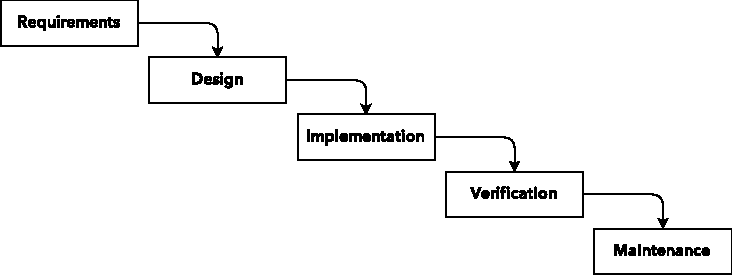
\includegraphics{figures/waterfall-model}

    \caption{Waterfall Model}
    \label{figure:waterfall-model}

    \vspace{1cm}

\end{figure}

Software development processes began to form. One of the primary functions of software processes was to determine the flow and order of how software is developed in stages~\cite{Boe88}. Notably in 1970, Winston W. Royce published a paper that described a formal approach for sequentially developing a software based on previously used practises~\cite{Roy70}. It was only later named as the Waterfall model~\cite{Boe88, LB03}. See figure~\ref{figure:waterfall-model}. The process consists of multiple stages that should be carried after the previous has been reviewed and verified. It begins by mapping the requirements for the entire software, then proceeding to designing the architecture, followed by implementing the plan, verifying the result is according to the set requirements, and finally maintaining the product~\cite{Roy70}. Generally, all this is considered as a linear timeline with a start and end. Each stage is planned and documented thoroughly. The concept thus being that as each step progresses, the specification of the software becomes further detailed.

However, contrary to what has been referred, Royce presented the model as a somewhat flawed, non-working model~\cite{Roy70}. If any of the stages fail, serious reconsideration of the plan or implementation might be necessary. Therefor sequentially following the stages would not produce what was intended and inevitably previous stages would need to be revisited~\cite{Roy70}. Royce however found the approach fundamentally sound and proposed the method should be carried out twice~\cite{Roy70, Boe88}. It should begin by creating a prototype and only then proceed in executing it. Nevertheless, this was overlooked and the single pass Waterfall model became the dominant software development process for software standards in government and industry~\cite{Boe88, LB03}. It is still used widely in some fields. It is noteworthy to mention that Royce has later been stated as a supporter for iterative approaches~\cite{LB03}.

Engineering methodologies, also called as plan-driven methods, are considered heavy. They also have not been noted for being terribly successful~\cite{Fow05}. The Waterfall model has been criticised as too linear, controlled, managed and documentation-oriented~\cite{Boe88, LB03, Fow05}. Waterfall pushes high-risk and difficult elements towards the end of the project~\cite{VB09}. Royce considered a software completed only when in addition to its implementation the documentation of it was acceptable — sometimes hundreds or even thousands of pages~\cite{Roy70}. It was declared that developers should prioritise keeping the documentation up to date over everything.

More lightweight iterative processes were proposed as opponents for sequential software development in the later part of the nineteen hundreds~\cite{LB03}. In fact, early applications of iterative and incremental development dates as far back as the mid-1950s — with many names such as incremental, evolutionary, spiral and staged development~\cite{Boe88, LB03, Fow05}. All of these sought in developing a useful compromise between no process and too much process~\cite{Fow05}. They also focused to be less documentation-oriented and in many ways more code-oriented. It was considered that the documentation for a project should be the code itself, not some external specification.

Fast-forward to 2001, when a group of software developers met to discuss new lightweight development principles. As the result of these discussions, a manifesto for Agile software development was published~\cite{BBB01a}. Four principles were proposed for Agile software development: \emph{focusing on individuals and interactions} over processes and tools, \emph{focusing on working software} over comprehensive documentation, \emph{focusing on customer collaboration} over contract negotiation and \emph{responding to change} over following a plan. The manifesto does not dismiss the value of the latter, but considers the former even more valuable~\cite{BBB01a}. From thereon, iterative processes have started to gain mainstream traction in the field~\cite{LB03, Fow05}.

Software development is now considered as an ongoing process, where a product should be build in small increments, iteratively going through the development stages. Repeating this process as long as required. Software delivery moved from a linear approach to a more recurrent cycle. See figure~\ref{figure:iterative-development}. The notion is not to resist change. Most of the ideas were not new and had been successfully used already in the industry for a long time before the manifesto~\cite{Fow05}. At that time, an urge revived to treat the ideas more seriously. Instead of planning, designing and implementing a whole software once, a software should be build iteratively by repeating all of these steps in shorter more controllable parts. Hence, any issue or miss-communication could be discovered early on and fixed accordingly.

\begin{figure}[h!]

    \vspace{1cm}
    \centering

    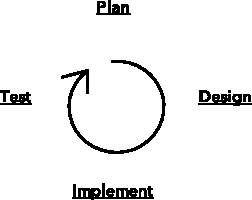
\includegraphics{figures/iterative-development}

    \caption{Iterative Development}
    \label{figure:iterative-development}

\end{figure}

\subsection{Adapting to Change}

The demands for software products are continuously shifting. It is not always obvious what the users want. In some cases, users do not know what they are looking for, until you show them what they need. It is hard to know what the value of a feature is before you see it in reality~\cite{Fow05}. Reality allows the user to learn how a feature works. An average client has little knowledge on how software products work or how they are built. Therefor, it is exceedingly difficult for a client to map specifically what they require from a software product. Software development should be more people-oriented than process-oriented~\cite{Fow05}. This requires a different kind of relationship with a customer. In most cases a user can be considered as the customer. What is notable, even Royce emphasised, although loosely, the value of customer commitment during development~\cite{Roy70}.

In most cases, rigorously planning a software beforehand will not work~\cite{LB03}. It is not uncommon that an idea will change quite a bit during its lifetime. The key problem that plan-driven  methods face is the separation of design~\cite{LB03, Fow05}. The concept is similar to traditional engineering: engineers will build a precise plan which will then be followed by a different set of people. In such, architects and engineers would first design a bridge and then a construction company would build it. A classic example is how Henry Ford standardised car parts and assembly techniques so that even low-skilled workers with specialised machines could manufacture low-priced cars to the masses~\cite{Pop02}. This lead to an explosion of indirect labour from production planning, engineering to management. All of this required a lot of overhead~\cite{Pop02}. Designing, which involves creative and more talented individuals, is far more difficult and less predictable than construction~\cite{Fow05}. Commonly expensive as well. Construction on the other hand, although more labour intensive, is considered more predictable and straightforward after a plan has been completed. The premise is that by following this methodology in software engineering, we could reasonably predict the time and cost of software “construction”.

When Royce first defined the Waterfall model, he stated that the documentation of a software is both its specification and design~\cite{Roy70}. Without documentation, there would be no design nor communication. Still to this day, no one has found a solid way of designing software in a manner that the plans can be thoroughly verified before construction~\cite{Fow05}. A design can look good on paper, but be seriously flawed when you actually program it. When building a bridge, the cost of the design is fractional to the cost of construction~\cite{Fow05}. It was thought beneficial that “low-skilled” programmers would produce the code, while a few “talented” architects and designers did the critical thinking~\cite{Pop02}. Naturally, this lead to a Waterfall-like process with different people involved in different stages. In software, the time spent implementing is fractional to the time spent designing. Essentially, coding is designing. Coding requires creative and talented people. People are considered one of the most important factors in software development. Developers should be in control of all the technical decisions. There are serious flaws in separating different tasks to different “specialists”, but this is how software engineering was regarded as~\cite{Roy70}. It is still quite common that a developer writing the code and a tester writing the tests, are not the same person. Even though studies have indicated that developers familiar with their own implementation tend to write more thorough tests~\cite{MND09}. The metaphor for traditional engineering is in practise flawed~\cite{Fow05}. Many projects simply fail in what they are trying to achieve and as a consequence the results will never be used~\cite{LB03}. Some reports have indicated that one of the top reasons for project failures is related to Waterfall-practises~\cite{LB03}.

Andy Whitlock, a product strategist, drew a fitting mental picture about changes~\cite{Whi14}. You see the road ahead as a clear and straight path to an objective you have set. What you do not always realise, is that the path will have its twists and turns along the way. What you can really only do, is to plan to a certain point ahead. The rest of your path will be a gloomy fog in the distance. You need to be ready to make difficult choices along the way. Agile development tries to create a framework, where processes and practises can take these requirements into consideration. Even to the point of changing the process itself~\cite{Fow05}.

\subsection{Being Agile}

Prominently, being “agile” means effectively responding and adapting to change and not resisting it. After all software is supposed to be “soft”~\cite{Fow05}. These course corrections are rapid and adaptive. The highest priority is to satisfy the customer trough continuously delivering valuable software from early on~\cite{BBB01b}. Software should be delivered frequently in short increments. These increments, also referred as iterations in Agile development, should take no more than a couple of weeks to a couple of months — the shorter the better~\cite{Fow05}. After each iteration a working software is delivered with a subset of the required features. These features should be as carefully tested as a final delivery. Throughout the project, one of the ways for a team to respond to change is by having effective communication among all stakeholders for the product daily. The best means for conveying information is face-to-face conversation — not documentation~\cite{BBB01b}. At every iteration the customer has control over the process by getting a look on the progress and then altering the direction as needed. This continuous feedback has been attributed as a key factor for success in agile projects~\cite{DD08}.

Commonly a stakeholder represents the views for the users or clients. By taking the stakeholders as part of the team, developers can react when something is not working as intended. The importance of customer reviews and acceptance was already noted in the Spiral model, which dates as early as the 1980s~\cite{Boe88}. Studies also show that developers see the ongoing presence of stakeholders helpful for development~\cite{DD08}. An Agile process is driven by the customer’s descriptions of what is required~\cite{BBB01b}. These requirements may be short-lived and that must be kept in focus. Changes are unavoidable~\cite{Fow05}. Users’ desires evolve and this must be harnessed to the customer’s competitive advantage~\cite{BBB01b, Fow05}. Even if deciding a stable set of requirements would be possible, outside forces are changing the value of features too fast~\cite{Fow05}. It is not uncommon for requirements to change even late in development. If you cannot get a fixed set of requirements, you cannot get a predictable plan. This is what makes plan-driven development inefficient. Royce stated that required design changes can be so disruptive that the software requirements upon which the design is based on and which provide the rationale for everything can be breached~\cite{Roy70}. Even so, predictability is highly desirable~\cite{Fow05}. It is an essential force in what makes a model work. Adaptivity is about making unpredictability predictable. This creates a framework for risk-control in the project.

One key premiss for Agile development is to reduce the burden of the process. Working software is the primary measure of progress~\cite{BBB01b}. A process should not hinder the work of a team — on the contrary it should permit the team to function to its full extent. By organising the team to be in control of the process, the framework facilitates rapid and incremental delivery of software. Still, no process will make up for the skill of the individuals working on the project~\cite{Boe88, Fow05}. Projects should be based on motivated individuals~\cite{BBB01b}. Motivation is maintained by creating a constructive environment and giving the necessary support when needed. Trusting the team is of utmost importance~\cite{BBB01b}. Morale has direct effects on the productivity of people~\cite{Fow05}.

One of the weaknesses of adaptability is that in its essence it implies that the usual notion of fixed-priced software development does not work~\cite{Pop02, TFR02, Fow05, HAB12}. Instead completely new approaches have to be used. Contracts should allow incremental deliveries which are not pre-defined in the contract, yet still ensuring the customer receives business value~\cite{Pop02}. You cannot fix scope, time and price in the same way as plan-driven methods have tried. The usual agile approach is to fix time and price and allow the scope to vary in a predetermined manner. Value is not only created by building software on-time and on-cost, but by building software that is valuable to the customer. Yet, value unquestionably still is a philosophical problem.

\subsection{Ensuring Quality}

Assuring quality is not an easy task. Applying measurements to software development is demanding. Something as simple as productivity is exceedingly hard to quantify. Let alone defining the value of something — from monetary significance to anything like user interpretations. ISO 9000 -standard defines quality as the extent of how well the characteristics of a product or service fulfil all of the requirements, the needs and expectations, set by the stakeholders~\cite{ISO9000}. IEEE defines software quality as the degree to which a system, component or process meets the specified requirements as well as the customer’s and user’s needs or expectations~\cite{IEEE1074}. Both definitions focus strongly on fulfilling the user’s needs. In this sense, quality and value have similar interpretations. It is also relatively hard to distinguish what is success, most of times this is based on the impressions of the people involved though sometimes some kind of measurement can be used as an indicator. Most of times these are focused on time and monetary value.

Software development is challenging. Users perceive quality as working software, but most of all emphasising good technical design and implementation makes the development process easier. People, time and money are limiting factors for ensuring quality. Strict deadlines and scarce resources have direct effects. Furthermore, human factors play a considerable role~\cite{DD08}. Several empirical studies reinforce the significance of Agile development processes and practises as improving quality in software~\cite{DD08, SS10, DNB12}. Evidently being “agile” should in the long term make development more predictable and eventually lead to shorter development times and minimised costs~\cite{DD08}. This provides an environment for being adaptive.

In addition to focusing on satisfying the customers needs, Agile development promotes continuous attention on technical excellence and good design practises~\cite{BBB01b}. Even so, this should not be accomplished by hindering simplicity. Simplicity maximises the amount of work that can be accomplished. The Agile Manifesto states that the best architectures, requirements and designs emerge from self-organising teams~\cite{BBB01b}. After regular intervals, the team members reflect on how they have performed and how they can become more effective. This is how the team can then tune and adjust its behaviour appropriately. The problem with traditional engineering is the separation of responsibility~\cite{Pop02}. Employees are not expected to take responsibility for the quality of a product. By giving responsibility back, you add accountability to the process. Developers will take quality more seriously.

Achieving quality is above all an ambition. No process or practise will account for quality if the developers are not willing to pursue it. A team must set mutual working principles which define how development will aim to deliver quality. These include anything from coding conventions to reviewing each other’s work. Quality should be a concerted effort. Above all, in addition of partly being a quantitative metric, value is qualitative.

The Agile practises also have their critics. Firstly, there is a lot of preconceptions about being Agile mostly driven by seeing the process as supporting no design nor documentation~\cite{HMP12}. Secondly, one of the biggest criticism is that there is a shortage of scientific support for many of the claims made by the Agile community~\cite{DD08, DNB12}. However, empirical studies have shown favourable results and studies have increased significantly~\cite{DD08, SS10, DNB12}. Agile development has been critiqued for a lack of focus on the architecture and design behind software. Practises are also rarely applicable by the book and therefor they are rarely used as such. Additionally, Agile development has a strong focus on small teams and as such many have struggled in seeing them used in larger distributed environments~\cite{TFR02}. One of the key concern has been also how to handle subcontracting which tends to lean heavily on documentation. Regards to embedded systems, there is issues in adopting Agile principles and practises to safety-critical environments~\cite{TFR02}. It is no surprise that it takes time and effort to introduce the methods properly~\cite{DD08}. In most cases, once you get past the first obstacles many of these hurdles are not an issue.

\subsection{Processes and Practises}

Processes and practises assist the development process. They create the framework and guidelines within a team can develop a suitable environment to deliver software~\cite{Kni07}. Martin Fowler discusses about a process as a part of the design~\cite{Fow05}. Processes and practices also help to maintain quality. Agile development has become well known and organisations are showing interest in adopting these methods~\cite{DD08}.

At the low level, developers use source code management to keep track of changes to the software and to collaborate with other team members. Source code management enables multiple developers to work on a single project, while also creating a history for the entire project. When a problem arises, developers can go back in time to look at the source code at any given point in time. To ensure features work as intended, developers use automated test cases to verify expected behaviour. There is a clear correlation between higher test coverage resulting in fewer errors in software~\cite{MND09}. By and large, writing tests for code has a better chance of signalling errors than untested code. Teams can also use more social methods — such as reviewing each other’s code — to validate the implementations. Pair programming, coding dojos and hackathons provide tools for improving skills and solving complex problems together~\cite{DD08, HHL13, RKD13}.

Most iterative development processes vary by the iteration length and how iterations are time-boxed — from a couple of weeks to a couple of months~\cite{LB03}. Agile development only provides a framework for software delivery. It does not specify concretely how development should be organised. Instead, development methods are incorporated to give focus on how software should be develop. Most notably, Scrum and Extreme Programming have created a structure for Agile development~\cite{LB03, Fow05, SS10}. Scrum provides a framework for managing development. It focuses on how development should be planned, managed and scheduled. It does not provide any strict practises, instead it gives guidelines for how customer requirements should be discovered, prioritised, and how the development of these features is split into iterations.

Scrum has been strengthened with ideas and practises which focus on simple design, small releases and coding standards. These also include test-driven development, refactoring, pair programming, collective ownership of the code, utilising on-site customers and continuous integration. These are defined in Extreme Programming~\cite{Bec00}. Continuous Integration aims at creating a process where developers integrate new features in small chunks and as often as possible into the software. In test-driven development, features are developed by writing the expectations for a feature as tests before actually implementing the code. When possible, code should also always be refactored to improve existing implementations. In pair programming, developers develop features in pairs.

Extreme Programming practises have been easier to be studied than management processes such as Scrum~\cite{DD08, DNB12, KRM13}. Most of the practises have been regarded as improving the quality of software and most developers tend to support them~\cite{DD08, SS10}. What is more, these practises make software development progress visually and aurally available. This increases the confidence that you are building what users want. Teams also improve the quality of their work: communication and understanding is improved, knowledge is transferred among the team and developers are more confident about their work. This increases morale and productivity~\cite{SS10}. A productive team is a right mixture of talented people. A team will not work if its members cannot work together. Regardless, it is still clear that many of the practises need more empirical studies to validate their claims~\cite{DD08}.

\subsection{From Agile to Lean}

As time has passed, developers have simplified software delivery even more. Agile has turned into Lean. Popularised, being “lean” means reducing the amount of “waste” around software development. Craig Larman and Bas Vodde have criticised this simplification~\cite{LV09}. Above all lean thinking is defined by respect for people and continuous improvement (kaizen). You need to challenge everything and embrace change. One way to achieve this is to remove anything from the process that does not have benefit. Some principles for Lean development are: \emph{eliminating waste, amplifying learning, deciding as late as possible, delivering as fast as possible, empowering the team, building integrity in and seeing the whole}~\cite{PP03}. Lean refers to an approach in manufacturing that was originally developed by Toyota in the 1950s~\cite{Fow08}. It became well known for the rest of the world in the 1990s when westerners started to explore why Japanese where leading in so many industries. Principles of lean thinking are universal and have been applied successfully in many disciplines~\cite{Pop02}. Many of the ideas presented by Lean Manufacturing have influenced the roots of Agile in software development. Both place notable attention on adaptive planning and people-focused approaches. In recent history, the software community has started to embrace Lean principles with more clarity~\cite{Fow08}. Agile and Lean are deeply entwined — you are not only agile or lean, you are both agile and lean.

Lean emphasis doing work just-in-time, not too early and not too late. Instead of dealing with a lot of up front design, just-in-time delivers a better paradigm~\cite{Pop02}. The principle is to structure processes so that they do nothing but add value and as fast as possible. This is accomplished by removing unnecessary waste and moving decision-making to the developers. “Mass-production” requires immensive amounts of work to create a process that does not directly add any value. This takes time. Time that is of the essence. Being “lean” means reducing this framework to the minimum and providing customers value with significantly fewer resources. As a notable example, Pierre Omidyar created eBay by responding to daily requests for improvements to the service~\cite{Pop02}. Many of these improvements where integrated overnight.

Iterations have in some cases even turned into building single features at a time. The idea of time-boxed iterations has become less important, you build a single feature and once done continue to the next one. Instead of building a frame for a ship, a development process should essentially start with building a boat first. To evaluate an idea, developers should begin by developing a minimum viable product (MVP) to validate the implementation has value~\cite{Rie11}. The notion is that sometimes ideas can be evaluated quicker by implementing them rather than spending time with a committee to decide the requirements~\cite{Pop02}. Even Royce hinted on prototyping in the Waterfall model and later the Spiral model integrated this as a principal concept~\cite{Roy70, Boe88}. Only a minimal effort should be put into place to specify the overall nature of a product. Being “adaptive” has transformed into quantitatively assessing what effects changes have. This so called build-measure-learn cycle or continuous innovation has transformed how features are developed and validated~\cite{Rie11}. See figure~\ref{figure:build-measure-learn}. Either you change you heading by pivoting or you persevere with the choice you have made.

\begin{figure}[h!]

    \vspace{1cm}
    \centering

    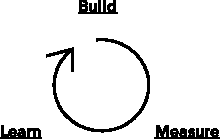
\includegraphics{figures/build-measure-learn}

    \caption{Build-Measure-Learn Cycle}
    \label{figure:build-measure-learn}

    \vspace{1cm}

\end{figure}

This mentality of continually innovating has become popular among software startups~\cite{Rie11}. An entrepreneur with a big vision and stubborn determination can charge through obstacles and make whatever their ambition is. The passion, energy and vision that people can bring to new ventures are resources that should not be disregarded. However, it is difficult to choose when to take a new direction. These decisions can be backed by anything from intuition to external indicators such as user feedback. In any case, making changes requires courage and determination. The build-measure-learn cycle makes it possible to test reactions, learn and iterate. Making decisions purely based on intuition can be risky. Learning, adapting and making changes are guided by data~\cite{Rie11}. It has even been suggested that experiments with negative user effects should be conducted~\cite{KLS09, KDF12, Bos12}. Still, personally I would argue that these experimentations need to be carefully planned. Not all users tend to agree with the use of somewhat unethical experimentation practises~\cite{RM13}. If a minimum viable product does not focus at all on the user experience, there is a high chance that users will seek for alternative options.

\subsection{Focusing on the Essential}

You eliminate waste by using activities and resources that are only absolutely necessary. Everything else is waste. The idea of doing things right has been widely misused as a justification for doing plan-driven development with heavy planning~\cite{Pop02}. Instead, software should be developed with short incremental cycles to ensure feedback and learning. This way, developers learn when something can be adjusted and most of all the customer can have direct effect. You concentrate on building features that will bring value by moving other decisions to as late as possible. Commitment should be delayed until there is certain demand that indicates what the users really want.

By delivering as fast as possible you ensure you can concretely see whether the feature has value or not. Development should centre on the people that have most effectiveness. Responsibility should not be transferred away from these people. Developers should have control on every part of the process. If something does not work, they have the chance to make a difference. Developers should challenge their skills instead of separating different tasks to different people. Maintaining responsibility and keeping a keen awareness and interest on the process builds integrity. All the skills required to build the product should reside in the team: from understanding the customers’ needs, to architecture, design, development, testing and management. When these principles are applied to software development you ensure you see the product as a whole. Fundamentally, Lean development tries to not hide the unknown.

Such as Agile development, Lean development is more or less a mindset. It emphasis certain aspects that guide development. Developers still have a lot of flexibility in how they utilise these guidelines in development. Lean development has also brought some popular practises such as Kanban, which is a visual way of organising work into tasks and limiting the amount of work currently in progress~\cite{Mon12}. These tasks are for example written down on sticky notes and their progress is made evident by moving them through different production stages: to do, doing and done (for example on a wall of an office).

% -- Deployment Pipeline --

\section{Deployment Pipeline}

Someone thinks of a good idea, but how do we deliver a feature as quickly as possible? In many software projects, releasing new features is a manually intensive process. Typically delivery of software to the users occurs at the very end of the project~\cite{HAB12}. Optimally, this should not be the case. Releasing software has a tendency to fail. Fixing major production issues after development can be hard to accomplish. How can we for example determine a software will work in its intended environment and not just on the developer’s machine?

A deployment pipeline is the foundation for many modern software development practises. Anything that can be treated as construction should be automated~\cite{Fow05}. One of the obstacles of build and test environments is that you want to be able to build fast so that you can get fast feedback~\cite{Fow13b}. Deploying software manually is a fragile and time-consuming process. Ideally a software should be able to be deployed by anyone with the simplicity of a push of a button. No struggle in finding out the steps to do so and automated ways in discovering if something has gone wrong along with rollbacking when this happens. To ensure quality, you have a comprehensive set of test cases for your code. Running these tests manually can take a long time. A deployment pipeline handles this by breaking up your build — with automated scripts and tasks — into multiple stages. Each stage increases your trust that everything is working as expected.

Jez Humble and David Farley describe three common anti-patterns for software delivery: deploying software manually, deploying to a production-like environment only after development is complete and manually managing production environments~\cite{HF11}. Most applications are rather complex to deploy and the process involves many moving parts. Eventually this leaves the process prone to human error. The purpose of a deployment pipeline is to provide automated and frequent releases of features. Any change in the software should trigger a feedback process. Features should be deployed so that developers receive feedback promptly and can act upon it. Features should be considered complete only when they are deployed to production~\cite{HF11}. Reflecting the ideas behind Agile and Lean development. The end result of a deployment pipeline is a production ready software or a cloud deployment. Without a deployment pipeline, development undoubtedly slows down. One is not truly incited to develop features incrementally.

\begin{figure}[h!]

    \vspace{1cm}
    \centering

    
\includegraphics{figures/deployment-pipeline}

    \caption{Deployment Pipeline}
    \label{figure:deployment-pipeline}

    \vspace{1cm}

\end{figure}

Typically a deployment pipeline consists of at least three stages: development, staging and production~\cite{HF11}. See figure~\ref{figure:deployment-pipeline}. Stages can be automated or require human interaction. A deployment pipeline begins by a developer implementing a feature and building the software. The pipeline runs automated test cases and other build related checks, but can also include manual checks that cannot be automated. These tests are also run in a production-like “staging” environment to be sure the feature will work once it will be deployed. The final stage is deploying the software to production. The purpose of a deployment pipeline is to detect any changes that will lead to issues in production~\cite{Fow13b}. In addition, it gives you visibility about changes in your development process. This visibility is easier to follow.

\subsection{From Development to Production}

Developing a software feature starts with the developer. Developers carry out ideas and turn them into code that implement a feature. Everything that is required to build an application should reside in a shared code repository~\cite{HF11}. This source code management keeps track of changes and makes it possible for several people to work on the same project. It also creates an invaluable history, where developers can go back in time and look through how the project has changed over time. This makes troubleshooting easier. A developer should be able to pull a local copy of the shared repository and with minimal effort — such as installing the required programming frameworks — get the application building and running. This should be an automated and straightforward process.

A developer should be encouraged to implement features in small chunks. Continuously integrating code is first of all a practise, not a tool~\cite{HF11}. Development practises require a degree of commitment and discipline from developers. Developers write code, related automated test cases and manually test that the feature is working as desired. This includes interacting with the actual software. After finishing, a developer runs all the test cases for the project. Thus making sure that any local changes have not broken something else in the application. Finally, the work is integrated back into the shared repository. In small chunks, even multiple times a day. Integrating code is about conveying information amongst the team. Other developers can see what has changed, test new features and make sure nothing conflicts with the work they are doing. This prevents any major integration troubles in the future. It is common that developers also have social practises for validating implementations. New features might not be integrated to the main branch before they are reviewed by another team member.

A local development machine is only a local setting. An application can seemingly work as expected on a local environment, but this must be verified against the production environment. Once the feature has been integrated into the repository, it is then immediately tested in a production-like setting, usually called as “staging”. A server runs the scripts and task related to building and testing the application. These include tests cases and any other checks that make sure the code is satisfactory. Tasks can include anything from analysing code style which include spotting human errors to verifying the test coverage. If anything fails, the developers should notice the issues relatively soon and fix them accordingly. The idea of a staging environment is to simulate the production environment. Tests should be run under this controlled environment to make sure the software works as intended in the desired final environment.

Finally, the last step includes deploying the application to production. It is not always feasible or desired to deploy software straight to production. Staging software adds a secondary barrier to verify the application. Customers can also see if the feature works as intended and any changes can still be made before deploying the feature to users. In web-application, features can even be deployed gradually starting from a subset of users~\cite{Bos12}. If this goes well, gradually more servers will be deployed with the new feature. At any point in time, the deployment can be rollbacked to a previous version if any issues are raised.

In addition, managing the staging and production environments should be made as easy as possible. The application stack should be easy to maintain and all related configurations should be in a repository~\cite{HF11}. Any developer should be able to create a production environment precisely, preferably in an automated fashion. Virtualisation and service-oriented platforms can help to achieve this.

\subsection{Continuous Integration}

Continuous Integration (CI) is a development practise where members of a team integrate their work frequently, usually multiple times a day~\cite{Fow06}. This leads to multiple integrations of the software every day. As described previously, each integration is verified by an automated build and test process to detect any errors as soon as possible. Less time is spent in trying to find bugs, because they are discovered quickly. Only if the source builds and tests without any error, can the overall build be considered good~\cite{Fow06}. If and when a developer breaks the build, it is their responsibility to directly fix and repeat until the shared state is functional.

The essence for continuous integrating is maintaining a controlled source code repository~\cite{Fow06}. Software projects involve a lot of files and manually keeping track of these is hard. Source code management allows developers to keep track of changes to the source code and to collaborate with other team members. Any individual developer works only a few hours at time from this shared project state. After the work is done, the developer integrates their changes back into the repository.

Integration is a way of communicating with the team. Frequent integrations let team members know about changes to the software. This eases any changes necessary in their work. Developers can also see if their work conflicts with any other team member. It also encourages developers the keep their work in as small chunks as possible. This significantly reduces the amount of integration problems by shortening the integration cycle and removing any unpredictability. Conflicts that stay undetected for weeks are hard to resolve~\cite{Fow06}.

The integration process is run locally, but in addition the process should be run on a separate automated integration machine, a CI -server~\cite{Fow06}. A build can be started manually, but most of the time this process is automated as soon as the developer integrates their work back to the shared repository. This prevents any flaws that might not be discovered on a local environment. On a CI -server, the build should never stay failed for long.

Continuous Integration assumes a comprehensive test suite for the software. The tests are a integral part of the integration and build processes which in affect results in a stable platform for future development. It is easy to add new features since it is easy to integrate and test them against previous functionality. An integrated system and well-tested software is key for bringing a sense of reality and progress into a project~\cite{Fow05}. Documentation can hide flaws that have not yet been discovered. Untested code can hide even more flaws. Practises such as test-driven development enhance integration by introducing programmers into writing simultaneously tests as they write production code. In addition, writing tests before the implementation is a design practise. Of course, you cannot count tests to find every single bug, but imperfect tests are better than no test at all~\cite{Fow06}. It has been stated that projects that use CI, tend to have dramatically less bugs~\cite{Fow06}.

\subsection{Continuous Deployment}

Continuous Deployment is a development practise where you build software throughout its lifecycle so that it can be deployed automatically at any given time~\cite{Fow13a}. Continuous Deployement requires that your pipeline enables you to do Continuous Delivery. The difference between Continuous Delivery and Deployment is that the first enables you to deliver new versions of your software easily with a push of a button whenever you so desire, instead the latter automates this process by doing deployments automatically to production, resulting in many production deployments each day~\cite{OR11, Sny13, Rub14}. The ability to delivery software functionality frequently to users subsequently enables to continuously learn from real-time usage~\cite{HAB12}. Usage data can be utilised throughout development, delivery and deployment. As a result the feedback-cycle becomes shorter.

You achieve Continuous Deployment by continuously integrating the features completed by the development team. Teams prioritise keeping software in a deployable state. Features are integrated, built and automatically tested to detect any issues. If no issues are raised, the software can be deployed automatically to production. Furthermore, you use environments that closely resemble the production environment to first see how the software performs before finally deploying it to users. By making small changes, there is a lower risk of something going wrong. When this happens, it is likely that these issues will be easier to fix.

The value of doing continuous deployments is that the current version of the software can be deployed at a moments notice without panic. Resources are not wasted in doing manual tasks. Deploying software frequently gives a sense of believable progress, not just developers declaring features done~\cite{Fow13a}. In addition of requiring extensive automation throughout the deployment pipeline, it also involves a close and collaborative working relationship between everyone from developers to system specialists involved in the software delivery process~\cite{HAB12, Fow13a}. Lately this has been referred to as a “DevOps culture”~\cite{Fow13a}. In practise, developers should have control on how software is hosted and this should not be primarily outsourced~\cite{HF11}. Developers can make appropriate choices based on these decisions.

Continuous Deployment also provides a way of making the latest version of the software being always accessible. Other developers and customers can then effortlessly demonstrate, explore and see what has changed since the previous version. It enables stakeholders to test the system and give feedback. A substantial risk in the effort of building something is whether or not it is useful to the user. The earlier you have the change of evaluating the value of a feature (MVP), the quicker you get feedback on it. Using the web has enabled the possibility to deploy and explore features on a subset of users~\cite{Fow06, Fow13a}. This can then be used as factor in making decisions about how to proceed.

\subsection{Continuous Experimentation}

Innovation is a moving force for organisations, but notoriously hard to get right~\cite{BE12}. The world is never static, being able to figure out what works and what does not can mean the difference between being on the top or becoming invisible~\cite{KLS09}. Innovation is maintained by balancing between the number of ideas presented and those being practical. The web has for example provided a platform for easily establishing a causal relationship between changes and their influence on user-observed behaviour~\cite{KLS09}.

In the simplest form of these controlled experimentations, users are randomly assigned to two different variants of a feature: a) the Control and b) the Treatment. The Control represent the existing version of the feature and the Treatment a new version being evaluated. At large this is called as A/B testing. Data is collected with predetermined metrics from these experiments — metrics such as how the user behaves with the feature. From these results we can determine by statistical analysis which implementation is better, although surprisingly not always why. Different implementations can have very unexpected results~\cite{KLS09, KDF12, McK12}. It is intriguing how poor we are at assessing the values of our ideas — many assumptions are simply wrong~\cite{BE12, KDF12}. Regardless of these assumptions having significant effects. Features are built because developers believe they are useful. Even worse, these opinions can come from managers not familiar with the area in question~\cite{KLS09, BE12, Bos12}. Of course, the significance of intuition and luck should not purely be belittled.

Controlled experiments provide a methodology to reliably evaluate the value of ideas~\cite{KR04, KLS09, McK12, Rho14, Wan14}. Passive feedback can provide much more valuable information than actively trying to ask feedback from users. Users can be blinded by how they act with features. By building a system for experimentation, the cost of testing and failure becomes small. This encourages innovation by enabling experimentation. Failing fast and knowing when an idea is not great is essential in making course corrections and developing better ideas. When we fail fast, we can also make improvements more faster. Due to the distributed nature of the web, these experimentations can be done in the background. New versions of features can be deployed frequently without the user even noticing the changes. This provides a thriving environment for experimentation. Experimentation can be used to understand what these user truly want~\cite{Wan14}.

Continuous Experimentation is a development practise where you build an environment where you can continuously deploy new features and enhancements to the user~\cite{FGM14}. As a result, developers can continuously get direct feedback from the user by observing usage behaviour. This requires an environment where you automatically deploy new features, collect metrics from usage, analyse them and furthermore integrate the results into the development pipeline. Instead of heavy up front testing, alerts and post-deployment fixing should be tried~\cite{FGM14}. When an issue is discovered, the feature can be rollbacked promptly, sometimes even automatically. The adoption of cloud computing has clearly shown a different approach to adding frequent and rigorous experimentation to the development process~\cite{Bos12}. Continuous Experimentation makes substantial use of minimum viable products as the basis for an hypothesis and experiment. Choices are made by analysing the data gathered from this minimal implementation. A hypothesis is either supported by the data or not. It is necessary to base decisions on sound evidence rather than guesswork~\cite{FGM14}. Controlling every aspect of development will not work, instead you need to sustain a culture where teams can move and innovate with the experimentation system~\cite{Rie11}.

Indeed, the leading edge of Continuous Experimentation is even starting to favour experiments over predefined test cases~\cite{New15}. Instead of rigorously testing features beforehand, automatic analytics are run in production. Heuristics are used to immediately discovers issues and alert about their consequences. This is also referred to as Canary testing~\cite{HF11, Sat14}. (As cruel as it can sound, canaries where used to test whether toxic gases where present in coal mines~\cite{Sat14}.) Changes are rolled out slowly to a small subset of users before rolling out new features to the entire infrastructure. Used by companies like Google and Netflix~\cite{Whi11, Sch13}. Testing in production will be as production-like as it can be. Another variation of production-testing is Blue–Green deployment, where you maintain two practically identical production environments as a backup to enable hot-switching between two alternatives and even feeding some transactions to the blue variant and some to the green one~\cite{Fow10, HF11}. Lately, Continuous Experimentation has become popular among companies building web-products such as Etsy, Facebook and Twitter~\cite{McK12, Boh13, New13, Rho14, Wan14}.

\subsection{Using Web as a Platform}

People have barely touched the surface of what the web can provide. The acceleration of digital products and services means the web will become more and more irreplaceable for software-intensive products and services. Cloud computing has emerged as a new model for hosting and delivering services over the Internet~\cite{ZCB10}. Infrastructure has become more cheaper, more powerful and more available than ever before. This made many of the current practises impossible back in the day~\cite{Roy70}. The cost of infrastructure is becoming negligible~\cite{ZCB10, Bos12}. Cloud computing has made it possible for general utilities such as computing power and storage to be leased and released over the network when necessary. This is highly scalable and adaptive, mirroring many of the Agile and Lean ideologies. Organisation can start small and increase resources only when there is rise in demand. One of the key reasons is the simplicity associated with not having to deal with hardware constraints~\cite{BE12}.

Cloud computing uses a service-driven model. Typically, cloud computing provides three categories of services: infrastructure such as computing and storage (Infrastructure as a Service), platforms such as operating systems and software development frameworks (Platform as a Service) and on-demand software applications (Software as a Service)~\cite{ZCB10}. It is no surprise that many of these services have become platforms for the deployment pipeline. Amongst all, this movement has generated service-oriented platforms that provide many of the common functionalities involved in software delivery. There is clear trend for continuously testing and experimenting with new innovative functionalities and deploying these regularly to users~\cite{BE12}. Especially web-applications and services can be developed and deployed with ease. Collecting data is a well-established strategy~\cite{HB14}.

\begin{figure}[h!]

    \vspace{1cm}
    \centering

    \makebox[\textwidth]{ 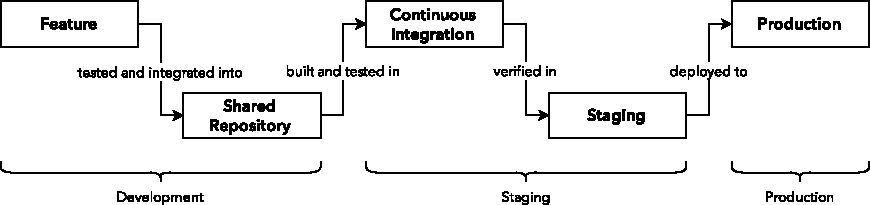
\includegraphics{figures/deployment-pipeline-flow} }

    \caption{Deployment Pipeline Flow}
    \label{figure:deployment-pipeline-flow}

    \vspace{1cm}

\end{figure}

Using cloud-based services has transformed software delivery: there is a fundamental shift in how products and services are developed and deployed. A popular paradigm nowadays is for instance to use GitHub for shared code repositories and project management, Travis CI for continuous integration and Heroku for web-application deployment~\cite{GitHub, Travis, Heroku}. Many of these services provide a high-level of interaction. A developer can push local changes to GitHub, GitHub can then start the continuous integration build on Travis CI automatically, and if successful the software can be deployed to Heroku. The use of cloud-based testing is accelerating: tests and analytics can be run post-deployment~\cite{RK14}. See figure~\ref{figure:deployment-pipeline-flow} for an example of a deployment pipeline flow.

% -- Towards Embedded Systems --

\section{Towards Embedded Systems}

Software is considered “soft”, hardware “hard”. Initially, software was only considered a convenient way to configure mechanisms for electronic systems~\cite{BE12}. It is not always obvious how products or features that combine software with hardware can be developed step-by-step. This combination, usually referred to as an embedded system, provides challenges in being agile and adaptive. Many of the Agile practises such as an identifiable customer, co-located development and minimal architectural design are outright opposite of what hardware-related embedded system development currently is~\cite{RA03}. There is a wide range of applications using embedded systems and the complexity and required functionality of these is increasing~\cite{KRM13, EHS14}. Intricate systems are getting increasingly difficult to verify and validate.

The industry has started to recognise that setting requirements for products is the most difficult and deciding part of the software development process. All of this requires new thinking on how hardware products are being developed. Eminently, this is why Agile and Lean philosophies are starting to get attention on the embedded field, not only for small organisation but for large ones as well. Prominently, while teams have succeeded in adopting Agile software practises, the organisation level is still governed by plan-driven approaches~\cite{EB12, EHS14}. Notably, a previous background in Agile and Lean practises seems to influence many of the development practises in embedded systems~\cite{KRM13}.

Nevertheless, there is still uncertainty whether the same agile ideologies and practises can improve the product development of embedded systems as much as they have reshaped the way user-focused software is being developed. Agile methods were not targeted for developing embedded systems where usually the object is not a person but instead a hardware. This manifests itself as limited customer–developer interaction. A development process tends to be focused on the integration of the whole product rather than being feature-driven. There are restrictions that are inescapable. For instance, it is not practical to develop a new working hardware prototype for each iteration. This does not alleviate the fact that experimentation is still required, because hardware constraints tend to have direct effects on later stages of development. Still, studies show that the use of Agile and Lean methodologies do have a positive effect also on the development of embedded systems by reducing development times and improving the overall development process and quality of products~\cite{CWR10, KRM13}. Agile methods can be used with success if the underlying restrictions are addressed accordingly~\cite{RA03}. Even Boehm observed in the 1980s that iterative development suited equally both software and hardware development~\cite{Boe88}. Lehtonen et al. researched agility in embedded systems particularly from the perspective of well-being at work~\cite{LTR14}. Using case studies, they conclude that increasing communication and being able to estimate workload evidently improve the meaningfulness, satisfaction and motivation of individuals.

\subsection{Embracing Agile Development}

It has become clear that methods and practises need to be adapted to suit each specific field~\cite{VB09, CWR10, HMP12, JLP12, KRM13}. There are also alterations of Agile that may be more suitable for plan-driven and large-scale environments, such as Scaled Agile~\cite{ScaledAgile}. There is no silver bullet. The wide diversity of products and their domain-specific problems are very distinct. No single method will work, but rather a combination of best practises need to be utilised. The research field on embedded systems is still very young and most of the input is coming from the industry, which in turn does not tend to share internal practises to the public~\cite{KRM13}. Some doubt has been casted on whether current Agile and Lean practises alone are sufficient in embedded settings — especially when related to safety-critical environments~\cite{TFR02, EB12}. Hardware-software systems are playing an increasing role in our everyday life making safety considerations a paramount concern~\cite{CWR10}. It is obvious though that agile and formal software development are not incompatible and features from plan-driven development can be adopted in iterative development. Agile practises such as test-driven development, early and exploratory releases and pair reviews support many of the requirements for formal development~\cite{TFR02, VB09, CWR10, JLP12}. Importantly, this provides a feedback-cycle for improving development.

The most explored Agile methods in embedded systems are unsurprisingly Extreme Programming and Scrum~\cite{KRM13}. However, many of these practises have different focuses than in “traditional” software development. A different focus makes sense, since the practises are considered mostly as a baseline for practical usage instead of rigid guidelines. For example in the context of embedded systems, refactoring may focus on making improvements to the speed, memory or power consumption instead of improving the quality of code. Sometimes resulting in even hurting the simplicity and clarity of the code. Performance and software reliability are key factors~\cite{RA03, EHS14}. Systems have to perform tasks within a defined time slot. Refactoring can even be risky, since hardware is very sensitive to changes in timing. Small changes can have somewhat large effects. Many of these effects are impossible to tell without hands-on experience with the hardware~\cite{RA03}.

Embedded systems have a dedicated function within a larger mechanical or electrical system. This requires hardware to accompany the software. An embedded system is a specialised computer-based system designed for a dedicated task or purpose. There is a clear distinction between embedded software and embedded systems~\cite{KRM13}. The former is constrained usually by restrictions set by the hardware, but the latter is not only constrained by the hardware itself, but also restrictions set by the development process of hardware. To simplify, an embedded software is part of an embedded system. An embedded software targets an existing system, whilst an embedded system involves building a hardware product from the ground up. I have set my perspective to emphasise not only the hardware aspect, but also the hardware development process as a key part of software development in embedded systems. Embedded systems can vary from mobile phones, cameras, robots to aeroplanes. Many of these systems require thorough planning and this is why plan-driven methodologies have been used widely. Even so, requirement changes are still very prominent, not all requirements can be mapped before starting product development.

Increasing requirements and unpredictability for embedded systems has led to the adoption of agile methods in hardware environments. Customer collaboration has become invaluable. Nonetheless, this is still a relatively new shift. Organisations have started to become more aware of the advantages that agility has brought to software projects, but the use of Agile and Lean practises is not widespread in the embedded field~\cite{CWR10, EB12, KRM13}. One of the biggest barriers on adopting new practises is organisational — mostly caused by conservative views~\cite{Pop02, HAB12}. Another big barrier is technical challenges related to the context~\cite{KRM13}.

A cultural change is essential~\cite{HAB12, KRM13}. Acceptance and knowledge of Agile methods are still rather limited in industrial settings related to embedded systems~\cite{HMP12}. The support for continuing with current plan-driven methods is conflicted with the desire to get the benefits from Agile practises. It is important to have a comprehensive view of the whole organisation~\cite{KRM13}. In a large organisation, it is not only sufficient to look at how single teams work, but how the organisation works as a whole. In current practises, teams are often well ahead of the organisation as a whole~\cite{HAB12}. An organisation should understand what they are trying to achieve with Agile and Lean methodologies. Not all companies should adopt practises the same way~\cite{KRM13}. As a solution, piloting and coaching new practises has been suggested to overcome resistance and convince on the advantages of iterative practises~\cite{CWR10, EB12, HMP12, KRM13}. Piloting can indicate what adjustments are called for adopting Agile practises within the organisation. People familiar with the practises tend to see the benefits more easily. Mental acceptance is crucial for Agile and Lean practises to work~\cite{HMP12}. Otherwise there is substantial risk that Agile practises will be adopted to suit plan-driven approaches and not the other way around.

\subsection{Integrating Hardware and Software Development}

A challenge in developing embedded systems is maintaining hardware and software development and integrating these together~\cite{EB12, EHS14}. Developing embedded systems faces the same challenges which were posed by seeing software development as an engineering practise. Software and hardware development are still rather separated. Larger organisations are struggling with aligning hardware and software development cycles and practises~\cite{EHS14}. Face-to-face conversation might not be sufficient and other means of communication are necessary~\cite{RA03}. Usually the hardware is not a major part of the software development until very late in the project~\cite{RA03}. Hardware development is more expensive and has longer lead times, i.e. how long it takes from initiation to the completion of production process~\cite{EHS14}. Different teams handle different aspects of the process: engineers design the hardware and developers the software. Furthermore, different people have different domain knowledge, which hinders the principle of shared responsibility~\cite{KRM13, EHS14}. Software development in embedded systems is mostly driven by the hardware~\cite{BE12}. An organisation is typically more experienced either in software or hardware development, balancing between these is a skill.

The Agile notion of moving all control to development teams is hard to accomplish. Hardware development should be deeply intertwined with software development. This has been referred as a hardware–software co-design. Developers and engineers should work on small teams more closely on systems to get the most out of Agile development. Clearly this requires cross-functional teams to transition to an agile research and development (R\&D) approach~\cite{HAB12, EHS14}. An engineering process should be transparent to all stakeholders~\cite{KRM13}. There is an apparent need for developing software and hardware simultaneously~\cite{RA03}. It is true that some of the architecture emerges through experience gained during development, but initial design cannot be avoided. Some organisations developing mass-produced embedded systems have been successful in allowing agility for individual teams to define their own ways on working to facilitate speed, shorter iterations and improving quality~\cite{EHS14}. A key issue is how companies scale these practises beyond single teams.

One the most common approach to develop embedded systems is to use an integration-centric approach~\cite{EB12, EHS14}. Commonly, hardware and software development are separated into two parallel streams and the work is later in development process integrated into a product. Early in the development, requirements are allocated to hardware and software components by a central engineering team. This is followed by multiple development teams implementing the requirements allocated to each component. The work of each team, hardware and software, is synchronised to a common project model. After the components are finalised, they are integrated together to form complete systems. Once this is completed, a system level testing can be conducted. At worst, this is were most of the integration problems are discovered. This cycle is repeated up to five times according to the project’s stages. Typically one integration cycle lasts at least six months, meaning that complete systems require lead times of multiple years. Software and hardware cycles have a very weak link between them. The culture is to focus on predictability by foreseeing activities months ahead. A prime purpose of this stage gate model is to ensure the feasibility of releasing large investments for the following stages after each stage completes. Essentially this results in a linear approach where teams are dependant on others thus forming bottlenecks. Typically the idea of introducing Agile methodologies is to try to increase the rate of new features being developed within this cycle — mostly in a module development phase. Above all, software development is driven by the hardware~\cite{EB12}. See figure~\ref{figure:v-model} for a typical approach for applying Agile development in an integration-centric V-model approach.

\begin{figure}[h!]

    \vspace{1cm}
    \centering

    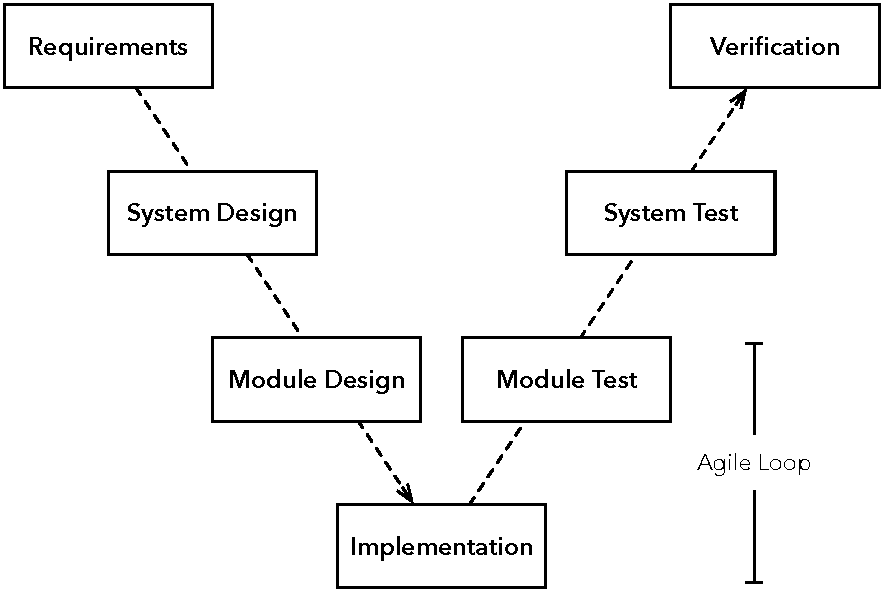
\includegraphics{figures/v-model}

    \caption{V-model~\cite{EHS14}}
    \label{figure:v-model}

    \vspace{1cm}

\end{figure}

Another key issue is that hardware and software development usually relies on many suppliers~\cite{EB12, HAB12, EHS14}. A situation that distinctly makes the development process complex. It is uncommon that an organisation can do everything related to hardware development in-house. Different suppliers provide components and factories combine them into hardware products. This also includes subcontracting different software components to different companies. Communication can be slow between all these moving parts. Not to mention difficult contractual matters. To get the benefits from Agile development and embrace shorter loops, all of these suppliers must follow similar principles and essentially abandon plan-driven processes.

Predictability may be desired in some circumstances. Organisations such as NASA are prime examples where software development must be predictable. NASA’s space operations consist of plenty of procedure, time, large teams and stable requirements~\cite{Fow05}. Having said that, NASA is also a prime example of an organisation where iterative development has been used with good results~\cite{LB03}. The challenge is to combine predictability with the dynamic capabilities of modern iterative development~\cite{EHS14}.

It is true that defining fully elaborated requirements work in certain applications where for example real-time systems and safety are important criteria~\cite{Boe88, KRM13}. At least some sort of top-level documentation might be required to support iterative development, most of times purely required by legislation, but also for managing and conveying information among the different levels of stakeholders involved in the project~\cite{KRM13, EHS14}. Regulatory standards can be rather rigorous, although they mostly do not impose any particular software development processes or practises~\cite{CWR10}. Traditionally safety regulations have been most regulated in medical, nuclear and avionics sectors~\cite{JLP12}. Lately, this has extended to automotive and railway sectors as the use of software has increased in these fields. Within the aerospace industry for example, nearly all Agile practises can be mapped to regulatory standards — albeit the industry has been slow in adopting them~\cite{VB09, CWR10}. This is also true for the railway industry~\cite{JLP12}. Though difficult, a transition is possible by incorporating and adapting Agile methods into existing processes~\cite{VB09}.

In embedded systems, the role of architecture and up front design cannot be avoided. In a regulated environment, there is a burden of proof which must demonstrate the compliance of the process~\cite{CWR10}. This makes it very rigid. It is imperative that there is full traceability throughout the development lifecycle. This obviously is a challenge for Agile and Lean practises. In any case, it has been suggested that Extreme Programming’s focus on test-driven development and the use of source control management can act as documentation and assist traceability. Also, Agile development in no way dismisses the importance of documentation. What it does emphasise however, is creating methods that make documentation easier to handle instead of making it a barrier for iterative and adaptive development. Organisations need to organise support for light-weight documentation methods such as issue trackers, wikis, whiteboards and even cameras~\cite{HMP12}. Some advocate using auto-generated documentation as much as possible~\cite{VB09, JLP12}.

\subsection{Historical Perspective}

History has many successful examples of the usage for iterative development in software development in embedded systems~\cite{LB03}. The X-15 hypersonic jet applied iterative and incremental development already back in the 1950s. In fact, the X-15 was only a hardware project. In the 1960s this knowledge was carried through to NASA, where iterative development was used in Project Mercury’s software. The project used surprisingly short iterations that only lasted a half-day. Interestingly, they also applied Extreme Programming practises such as test-driven development. Essentially, the platform for Project Mercury allowed the development team to build the system incrementally.

Later in the 1970s, the US Department of Defence used iterative development on large, life-critical space and avionics systems~\cite{LB03}. As an other example, the command and control system for the first US Trident submarine also used iterative development. Although, the project still used very long iterations taking as long as six months each. Other applications of iterative development included TRW/Army Site Defence’s missile defence systems and the US Navy’s Light Airborne Multipurpose System (LAMPS) part of a weapons system. The missile defence software project progressed by the team refining each iteration in response to the preceding iteration’s feedback, an early use of reflection and learning by doing. LAMPS was one of the earliest projects that used short iterations that only took one month per iteration. The project succeeded, deliveries were on time and under budget~\cite{LB03}. Notably, since many Waterfall project had fell short on this.

Another remarkable story is the primary avionics software for NASA’s space shuttle program in the late 1970s~\cite{LB03}. The motivation for using iterative development came from need to be able to handle changing requirements for the shuttle program during its software development. NASA used eight week iterations and these made feedback-driven refinements to specifications. In the early 1990s, a new-generation Canadian Automated Air Traffic Control System was developed using risk-driven iterative development. The project was also a success, despite its near-failure predecessor that applied the famed Waterfall model~\cite{LB03}. Still, it used rather long iterations of six months by modern standards.

Notably, all these examples are early examples of being agile, but it has to be said that they only applied a fraction of ideas presented by current ideologies. Recently Agile and Lean practises have been used with good results in the development of instruments, cameras, telecommunications software, health products, the automotive industry, automated vehicles and even aeroplanes and satellites~\cite{RA03, VB09, BE12, KRM13, HB14}.

\subsection{Using Hardware as a Platform}

Hardware is something concrete (sometimes even bare metal). Not only being something physical, but having many dependencies between components and the way they interface together. It is usual that hardware sets tight requirements for the software. The lifecycle of devices is measured in years, sometimes decades — resulting in many legacy platforms~\cite{BE12}. Obviously systems like traffic lights, railway signalling and ticketing systems for the Underground are upgraded rarely in contrast to for instance mobile devices. Maintaining these platforms requires legacy software and physical spare parts. Embedded systems need to evolve to stay attractive for users especially in sectors that are moving fast~\cite{BE12}. Product use evolves over time and features should be adjusted duly.

Most of the challenges regarding iterative development can be overcome by designing a platform that can be easily extended and modified for different needs~\cite{KRM13}. A principal obstacle is caused by the lack of a base product which can be improved continually~\cite{HAB12}. This also includes modularising the software into smaller more manageable components. Investing in hardware development is many times more expensive than investing in software — requiring immense amounts of effort~\cite{BE12}. Let alone the undertaking caused by deploying these systems to actual use. A single product should be customisable for different customers instead of developing completely separate products. Subsequently, hardware becomes a platform for delivering value with software solutions. Increasingly software has become the core for almost all hardware systems~\cite{BE12}. Software is the enabler for new innovation. Keeping the process “lean” and reducing the unnecessary can provide a competitive edge~\cite{CWR10}.

The benefits of the web and cloud computing extend well beyond web-applications~\cite{BE12}. Remote deployments are possible on embedded systems. Microprocessor-based architectures have made it possible to update systems with new software releases~\cite{RA03}. These architectures are combined with application-specific integrated circuits that are customised for a particular use. A current trend is connecting these systems, from cameras to cars, to the Internet, sometimes also referred as the Internet of Things~\cite{BE12, HB14}. This enables Continuous Delivery on embedded systems.

Helena Holmström Olsson and Jan Bosch state three issues: 1) post-deployment data is being used for new products rather than for improving existing systems, 2) post-deployment data is used for troubleshooting and support rather than for innovating new features and 3) post-deployment data is being used to understand operation and performance rather than for providing insight in individual feature usage~\cite{HB14}.

\begin{figure}[h!]

    \vspace{1cm}
    \centering

    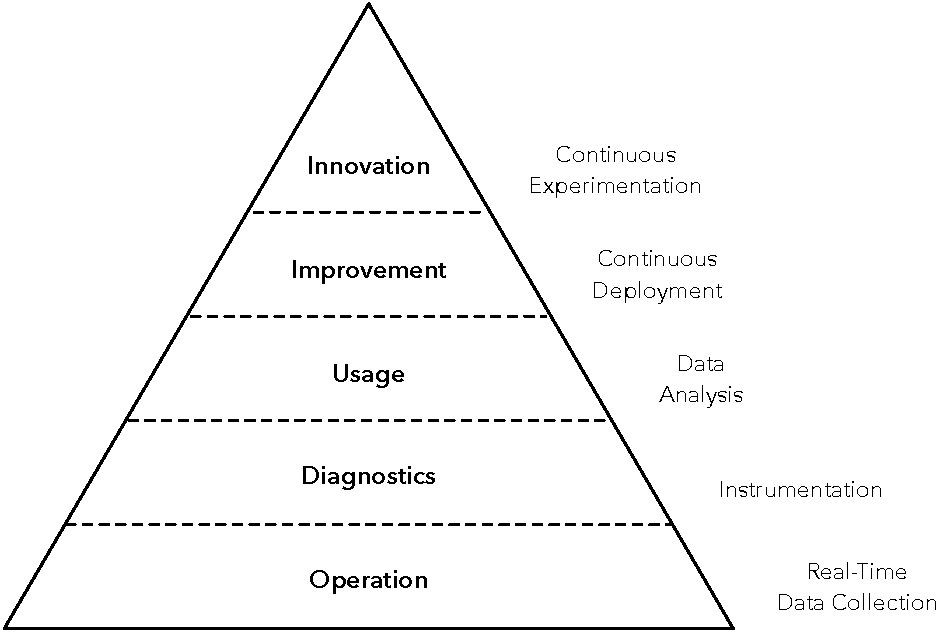
\includegraphics{figures/data-usage}

    \caption{Levels of Data Usage, adapted from~\cite{HB14}}
    \label{figure:data-usage}

    \vspace{1cm}

\end{figure}

Although cloud computing currently is applied in delivering software to the web, these techniques can be applied basically to any product that is able to collect and provide data about its usage — including even software-intensive embedded systems~\cite{BE12, Bos12}. See figure~\ref{figure:data-usage} for how data can be put to use. Data can be used in the research and development process of embedded products. This enables Continuous Experimentation on embedded systems. The organisation can spend time to developing the right things instead of fixing mistakes in needless functionality~\cite{HAB12}. By and large, organisation have significant quantities of data, but little is used for research and development~\cite{HB14}. For example cars can collect real-time fuel consumption data and telecom devices real-time bandwidth data~\cite{Bos12}. Previously these points of interest where only collected for management purposes, now data is used for development purposes as well. Still, post-deployment data is mostly used as input for development of successor products, but surprisingly not for improving features on current products~\cite{HB14}.

Service-oriented models have started to find their way to more embedded settings~\cite{BE12, Bos12}. Organisations are moving towards software-houses to be able to concentrate on bringing value through software. While high-quality hardware systems is still important, it is no longer the only differentiator between organisation and what makes a product competitive~\cite{EHS14}. In some cases, hardware products are being leased instead of them being expensive investments. Mobile phones and even cars are starting to take advantage of frequent, post-deployment updates to their software. Organisation are also interested in collecting usage and other performance related metrics. Instead of freezing requirements before starting product development, the requirements evolve and have effect on how users use the products. Users are becoming increasingly accustomed to frequent updates that add value. Consequently this also increases the expectations for users. Traditional static and unconnected hardware are fast becoming unsustainable. Upgrading is expensive and integrating new solutions involve risk and complexities that can be hard to predict.

In embedded systems, software is deployed as part of the overall system, including its hardware. Instead of servers, the software is deployed to the destination point. The process obviously requires changes to the architecture of the platforms to facilitate remote deployments and experimentation. Notably creating structures to collect data from performance to usage, analysing these, creating experiments and enabling remote deployments~\cite{BE12}. The ability to evolve and conduct experiences must be supported in a safe and controlled manner~\cite{BE12}. Jan Bosch refers to this as building an innovation experiment system, well suited for connected embedded systems~\cite{BE12, Bos12}. A research and development system responds to actual customer feedback collected from experimenting and testing features that the users actually need~\cite{HAB12}. Many embedded systems are deployed in customer locations. For that reason, there is demand for customers who can see the benefits for Continuous Experimentation and are willing to explore the concept in production~\cite{HAB12}. Furthermore, connecting devices to the Internet obviously poses security and privacy issues that must be taken account~\cite{BE12}.

New approaches such as electronic testing platforms like Arduino, 3D-printing and laser-cutting are bringing hardware development to the general public~\cite{Arduino}. Lately, it has become even possible to print circuit boards~\cite{Vol15}. Previously all these activities where limited to specific industries. Experimenting with hardware products is getting even more accessible. Microprocessor-based architectures can be rapidly expanded and used in a variety of different applications~\cite{KRM13}. Now, building a prototype for experimentation purposes is within reach.

\subsection{Adapting for Deployment Pipeline}

Embedded development is exploration-driven by nature: the development process includes extensive research and development resources~\cite{EHS14}. Still, testing is the cornerstone of embedded systems~\cite{RA03, HAB12, KRM13, EHS14, Ngy15}. Bugs tend to be hard to detect. Trying to detect whether they are caused by the software or hardware is demanding on its own. A bug might be caused by something completely not related to software~\cite{Ngy15}. Most of the software implementations need to be tested against the hardware since most of the code is dependant on it. Hardware development has slow development cycles, even lasting several years. Developer need to verify proper co-operation between the software and hardware. The more complex the interactions are, the more important experimentation is. That is why hardware simulation is an essential practise. This is problematic since test environments in the embedded domain have very different performance and memory constraints. Real-time requirements are hard to satisfy~\cite{RA03, HMP12}. Testing can take several days to achieve on actual hardware — if developers even have certified access to hardware environments~\cite{VB09}. The overhead of processes can make the lead time of simple bug fixes to several weeks. It is also common that stringent contexts such as aerospace need separate review teams~\cite{VB09}. In these contexts, developers have very strict access to only specific sections of code. Implementation and testing should be carried out by separate people to satisfy regulations~\cite{VB09, JLP12}.

The concept of running tests relentlessly on a target platform is hard to accomplish. Performance and memory constraints often prevent installing and running all tests on the hardware at the same time. It also takes significantly longer than say in modern computers. Anyway, basic usage of Continuous Integration is not hard to achieve in embedded settings — especially when related to unit testing~\cite{RA03, KRM13}. Integration and acceptance testing is harder to achieve. As with “traditional” software development, automatic testing will help to identify failures in an early stage. It will also increase awareness on what effect each build has on the overall system. People should not do the job of computers, Continuous Integration handles many error prone tasks~\cite{Ngy15}.

Organisations developing embedded systems are starting to seek for opportunities presented by Continuous Deployment~\cite{HAB12}. However, there is still a rather long leap for frequently delivering new features to users. Sometimes this is not even possible within internal processes. The need for both Continuous Integration and Deployment are well understood, but their implementation is unfortunately rather hard to accomplish without more deep changes. A key focus is for an organisation to develop a fully automated testing infrastructure to continuously verify development~\cite{HAB12}. Without a doubt, the distributed nature of web is a valuable platform for enabling remote deployments as well as collecting, analysing and experimenting with data.

With the high cost associated with testing new ideas, experimentation should be a well thought and simple process. Organisations are inclined to use observation techniques and expert reviews in pre-deployment research and development, but there is less evidence on organisations using methods focused on continuously collecting customer feedback~\cite{HB14}. Turning most promising ideas from concepts to prototypes should receive significant attention~\cite{BE12}. Iterating on features in embedded systems should be possible in short cycles pursuing Agile practises. Many current processes, such as the V-model, are focused in creating a process focused in rigid milestones to try to minimise losses instead of experimenting in small steps. An obvious cause for mundane innovation~\cite{BE12}. Instead organisations should focus on maximising the amount of iterations by reducing the related costs for each iteration. Post-deployment data can provide understanding of the operation and performance of embedded systems, but in addition how the user uses different features~\cite{BE12, HB14}. See figure~\ref{figure:towards-continuous-experimentation} for the steps related for moving towards Continuous Experimentation.

\begin{figure}[h!]

    \vspace{1cm}
    \centering

    \makebox[\textwidth]{ 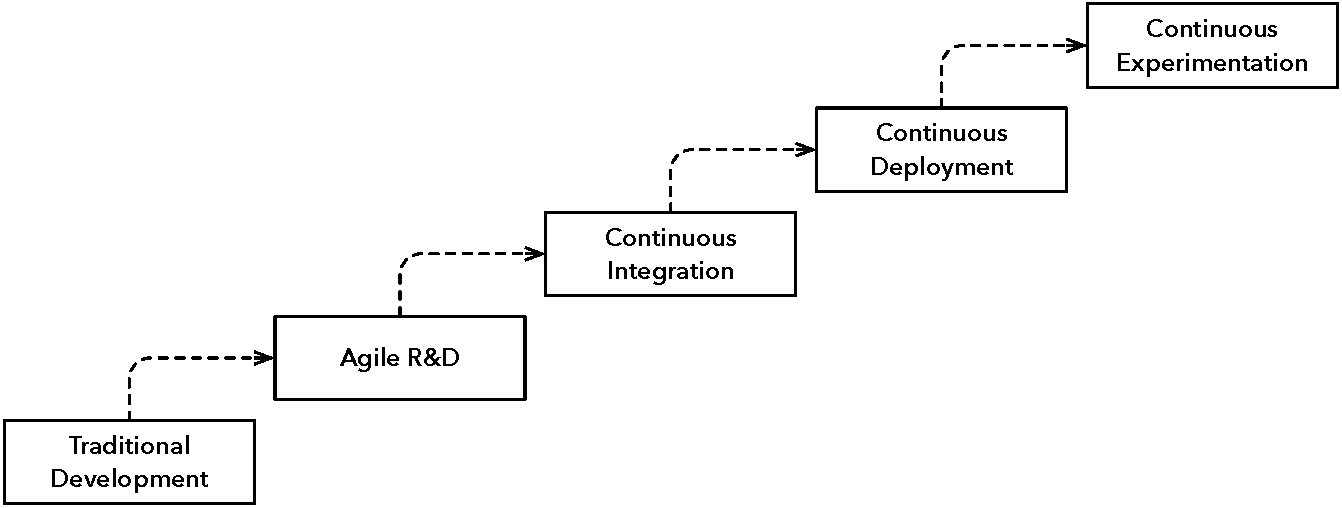
\includegraphics{figures/towards-continuous-experimentation} }

    \caption{Towards Continuous Experimentation, adapted from~\cite{HAB12}}
    \label{figure:towards-continuous-experimentation}

    \vspace{1cm}

\end{figure}

Specific solutions are required to mitigate the restriction in scaling the deployment pipeline in embedded systems. A special test environment may be needed in environments where the implications of feature changes are broad and the customer may have reluctance towards experimenting with new features~\cite{FGM14}. To avoid safety concern, Jan Bosch and Ulrik Eklund have suggested separating experimentation systems from the development of critical components~\cite{BE12}. Setting up an experimentation cycle can be rather challenging for developing software that requires hardware. Longer release cycles with hardware and potential synchronisation problems between the development schedules is an issue~\cite{FGM14}. An experimentation system can be used to guide research and development efforts~\cite{HAB12}.

In certain life-critical environments, experimentation can just be too expensive or undesirable to achieve~\cite{BE12}. Heavyweight sequential processes are outside of Agile research and development~\cite{EHS14}. Heavy verification and validation is required in contexts such as aerospace. This is why simulation becomes important~\cite{KRM13}. Simulation enables developers to work on software simultaneously while hardware is being evolved. Developers should be able to experiment by simulating in a production-like setting. The problem is that simulation is never really “production-like”. At least in the sense we are able to achieve in web-development. Software most likely will behave differently on the actual hardware.

At the leading edge, some organisation are even pushing web design philosophies to native applications to tackle the rigid environment of embedded systems~\cite{Boh13, GZ14}. In another example, the UC Berkeley Solar Vehicle Team is using Travis CI as a platform to test their embedded software that powers their solar vehicle~\cite{Ngy15}.

% -- Views from Embedded Settings --

\section{Views from Embedded Settings}

I conducted six semi-structured interviews with seven people working in the academia and industry on leading embedded systems to get a view on if and how Agile and Lean methodologies and the deployment pipeline has changed the development of embedded systems. The interview consisted of the following topics:

\paragraph{Process}

\begin{enumerate}

    \item Do you consider that your organisation follows the principles and practises of Agile and Lean development? Which of these principles have most significance?
    \item If so, has this recently changed the way you develop products or features into production?
    \item Do you approach development from the point-of-view of the whole product or by single features?
    \item Please describe the process behind developing an idea into a single feature. How long does it take?
    \item Do you recognise distinct development, staging and production environments in your process?
    \item If so, are these automated?

\end{enumerate}

\paragraph{Adapting to Change}

\begin{enumerate}[resume]

    \item How easy or hard is it to adapt changes in hardware related products?
    \item Can you deploy software changes automatically or even remotely?
    \item How do you keep software and hardware development in sync?
    \item How short iterations do you use to adjust for feedback from your stakeholders?

\end{enumerate}

\paragraph{Experimentation}

\begin{enumerate}[resume]

    \item Do you have an automated process for deploying or experimenting a feature?
    \item How do you experiment with software related to hardware?
    \item How do you value an idea (prototypes, minimum-viable products, A/B testing)?
    \item Related to hardware, has new approaches such as electronic testing platforms, 3D-printing or laser-cutting changed your process?

\end{enumerate}

Many of the mentioned topics and terms are prone to many interpretations. Thus their meaning is somewhat ambiguous. To address this, I started the interviews by introducing the topics and relaying my understanding on the concepts. This way we shared understanding on what I was trying to ask. I conducted the interviews both face-to-face on location and via email, which ever suited best for the situation. Each interview included additional discussion about interesting topics which arose during the conversations. Some of the interviews where more in-depth than others.

Most of the interviews are from European organisations or subsidiaries of multinational corporations in Finland. The participants include: Lauri Koivulehto from Airbus Defence and Space Oy, Stefan Baggström and Marko Taipale from GE Healthcare Finland Oy, Tatjana Petkovic from Space Systems Finland Ltd, Niklas Holsti from Tidorum Ltd and Harri Holopainen from ZenRobotics Ltd~\cite{Koi15, BT15, Pet15, Hol15b, Hol15a}. My interviews included also one participant from academia in Switzerland: Maximilian Kriegleder from ETH Zürich, Institute for Dynamic Systems and Control~\cite{Kri15}.

These cases cover a wide range of sectors from telecom, medical, aerospace to robotics. Representing the industry, Airbus Defence and Space Oy works in Finland in the telecom-sector, GE Healthcare Finland Oy produces health-care equipment and services, Space Systems Finland Ltd works on safety-critical embedded systems, Niklas Holsti has an extensive background in the aerospace industry in Finland and finally ZenRobotics Ltd works on waste sorting robots. As for the academia, ETH Zürich, Institute for Dynamic Systems and Control experiments among other things with intelligent quadcopters, Distributed Flight Array, famous from TED~\cite{Dan13}.

Be that as it may be, what is obvious is that the embedded field is very diverse. Different sectors and organisations have very divergent practises and opinions. No objective conclusion can be made for the whole industry and these interviews should be considered as inciting discussion rather than giving truths. In the following chapters, I approach the topics from three perspectives: process, adapting to change and experimentation. I also describe interesting views and findings presented by the interviewees. Some of the key findings include the challenges associated with developing embedded systems — varying for each context, but also having similar characteristics. The cases also present some interesting approaches adopted by organisations. Finally, I conclude with an overview of the interviews and present some smaller findings related to deployment pipeline.

\subsection{About Processes}

\epigraph{The Waterfall model has turned into a cliché that crumbles fast under inspection.}{\textit{Harri Holopainen~\cite{Hol15a}}}

According to the interviews, the notion of Agile and Lean principles and practises being suitable for the development of embedded systems is primarily accepted~\cite{Hol15a, Koi15, Kri15, Pet15}. Software and hardware development is a dialogue~\cite{BT15}. Yet there are some industries, such as flight related embedded systems in aerospace, where generally Agile development is not used at all~\cite{Hol15b}. This partly contradicts the previous findings from literature, albeit this can be caused by different interpretations~\cite{LB03}. In two cases, distinct Agile methodologies, such as Scrum, are used~\cite{BT15, Pet15}. One case has gone even further by adopting Lean principles as part of the organisational strategy~\cite{BT15}.

It seems, a plan-driven model is still more or less a consensus and widely used among many interviewed embedded sectors~\cite{Hol15b, Koi15}. However, this does not prohibit the use of iterative and incremental development within the surrounding process~\cite{Hol15b}. Holopainen considers that the Waterfall-model has turned into a cliché that crumbles fast under inspection — the surrounding world is not linear~\cite{Hol15a}. In fact, iterative development is being used at least to some extent along plan-driven methodologies, something that can be considered iterative plan-driven development. As common, many of these plan-driven methods do not stay generally on schedule or budget, mostly because requirements are finalised too late~\cite{Hol15b}. Holsti does not see the existing plan-driven processes to be of blame, but rather the reason lies in the inexperience of customers in underestimating the amount work necessary~\cite{Hol15b}. Yet, what is obvious among all interviews Agile or not, is that most embedded products are being developed from the point-of-view of the whole product with an emphasis on an overall picture. Even so, a wide adoption of Agile and Lean principles and practises is planned in most of the interviewed organisation currently focused in plan-driven approaches~\cite{Koi15}.

What is obvious, is that due to the very different environments, spotting distinct deployment pipeline practises is indeed hard. Each organisation uses different practises to deliver software to production. Software processes form under pressure from clients and environments~\cite{Hol15a, Hol15b}. Methodologies range from plan-driven methods such as the Waterfall and V-models to Agile and Lean implementations~\cite{Hol15b, Koi15}. In one case relating to the academia, no distinct process was used since the project was merely focused on experimentation~\cite{Kri15}. Some automatic deployment pipeline practises can be used in the development and production stages~\cite{BT15, Hol15a, Hol15b, Koi15, Pet15}. Most of these relate to using Continuous Integration practises, such as source control management, automated testing and static analysis of source code. Also social methods, such as peer reviewing are used~\cite{Hol15b}. Continuous Deployment is possible, but utilised to varying degrees~\cite{BT15, Hol15a, Hol15b, Koi15}. For GE, Continous Delivery is being used in software products~\cite{BT15}. Yet currently, some modern deployment pipeline practises, such as experimentation driven testing, popular from modern web-development have no straight equivalent in the processes used to develop embedded systems. The overall flow is not as automatic: testing procedures are somewhat manual, deploying features to production is slow and requires distribution and experimentation practises focus on the pre-production design phase instead of post-deployment. Individual components are there, but no where near as stable and connected than in web-development.

Where Agile methods are suitable, work is driven by customer and end-user needs — as well as views on future needs~\cite{Pet15}. In the case of Space Systems Finland Ltd, a typical lifecycle of a feature is: recorded, prioritised, assigned to a “work package” (sprint) and finally implemented with unit and acceptance tests and released. Corresponding knowledge on how Agile development is organised. Hardware development follows the similar stages and this can be accomplished due to extendable platforms. So far Petkovic mentions they have been able to develop hardware iteratively without significant troubles~\cite{Pet15}. According to Petkovic, the most significant Agile and Lean principles are those emphasising customer collaboration and flexible planning. The development follows short iterations varying from a few weeks to several months depending on the features priority which is decided by the (end-)customers needs. The overall process follows Agile and Scrum, but not fully~\cite{Pet15}. Progress meetings are held weekly, not daily. Although emphasis is still on communicating and exchanging ideas daily whenever necessary. A customer is involved even daily, usually weekly. Relating end-users, the feedback-cycle varies on the urgency — anything from daily to a few months.

When reflecting on hardware development, Koivulehto considers the processes are in good shape for instance relating to integrated circuits~\cite{Hol15a}. Indeed, really complex logic can be incorporated inside circuits, but the software and hardware placed of top of these is rather limiting. What is lacking is piecing intricate hardware development together with software development to build products as whole. Typically hardware manufacturing is modular and this works well. Hardware can be built by integrating existing components to get the desired functionality. When developing embedded software, the case is not the same. The field lacks of existing modular software implementations to interface with hardware~\cite{Hol15a}. Most software functionalities have to be build from the ground up. Again, an opposite of how web-development can be achieved with an abundance of existing frameworks.

According to Holopainen, iterative and incremental development is the only way to do development if the definition and requirements of what you are trying to accomplish are missing~\cite{Hol15a}. In every project, the essential problem is to determine the requirements. An increasing amount of customers understand the problem, but phrasing desires remains a problem. Agile development suits a context where the problem can be split into sections. Relating to web-development, many of the existing problems have been solved many times. Web-development is an ideal context for Agile development. A short feedback-cycle is an immense resource. Iterating is supported by data that can even be used to analyse what features bring most value. Unfortunately, Agile development is way ahead of how embedded systems are developed. Regardless, as such the bad attributes of the a context are not a fault of Agile development or a reason to not utilise it.

\subsection{A Stringent Context}

As a stringent example, the aerospace industry takes great lengths to supervise and manage change — evidently a reason why plan-driven methodologies such as Waterfall and V-models are being extensively used~\cite{Hol15b}. One simply cannot experiment with launching a satellite to space with flimsy approaches. Controlling change is a significant part of software projects in this critical industry. The industry is regulated and the quality of software projects is evaluated throughout the process with standardised processes. Typically, these plan-driven methods are not however linear. Not all requirements can be determined up front and iteration is needed throughout the process. Single teams and developers can work with even short iterations implementing features. What is key though, this iteration is handled within Waterfall-like processes. Therefor the V-model is generally used, since it focuses on a process where gradually refined requirements are accompanied by gradually increasing validation, enabling the use of some iteration. Requirements and software implementing these is delivered incrementally, part by part. The whole process can take up to several years. Hardware and software development are highly separated and embedded systems are being developed by subcontracting software for specific components of space equipment.

Subcontractors working on the software of embedded systems are on the bottom of the development chain — there is no doubt this requires considerable amounts of documentation for communication~\cite{BT15, Hol15b}. Procedures around documenting and reviewing requirements are extremely rigorous~\cite{Hol15b}. To be Agile, the whole chain would need to be agile. Software producers implement software for fairly set requirements at a fairly set price. In principle, the customer tries everything to minimise additional costs generated by changing requirements. Essentially this has axed out the ability to be even agile and experiment~\cite{Hol15b}. These stringent requirements have created standardised processes in the aerospace industry, which expect that the need for change comes solely from customers and is not formed by experimentation conducted by the developers. Change requests and their effect is thoroughly documented and integrated into the plan-driven process. In essence, a process must stay intact to be verifiable~\cite{Hol15b}. Holsti does note still that requirements tend to see a lot of smaller and even larger refinements~\cite{Hol15b}. These have effects on every single stage of the process. Essentially the plan-driven method is repeated multiple times throughout the lifecycle of the program, therefor resulting in iteration and incremental delivery of features. Most of these changes are caused by refinements in the hardware of the embedded system. A customer can also become aware that something in the hardware is not working as previously expected. A small change in the hardware can require alterations in multiple tiers of the software components~\cite{Hol15b}. These changes do not only have effect on how a feature works, but a small change can also have peculiar effects on the hardware itself: for instance changes in software workload can cause the voltage on the hardware to spike resulting in unreliable operation.

Yet, almost without exception, software for embedded systems in space equipments is developed in stages that represent the needs presented by the customer~\cite{Hol15b}. Often a dominant factor is that a hardware platform matures in phases. Hardware is being developed and built in separate components and these are then assembled at different paces according to the schedule of the overall project. Almost always, the hardware is assembled by the customer who subcontracts the software development. Only some core parts of the software are built in-house. A software producer rarely has access to the necessary clean rooms\footnote{In aerospace, hardware is assembled in clean rooms, where the environment has a low level of pollutants such as dust.} or knowledge required for this process. Developers do not have a chance to experiment with different software approaches, nor do they have the equipment to do so. Ultimately, the whole product is integrated in the customer’s location. Developers implement software features required for each specific assembly- and testing stage in very confined settings. What developers can do, is to test features by simulating the hardware, since most hardware does not even exist during development of software components. This can be accomplished either by specific hardware platforms for simulation or simulators based entirely on software. Simulation also enables to instrument and debug how the code behaves. Acceptance testing is based on the customers requirements and is specified early on the development process — typically side-by-side to programming. Unit tests are derived also from the customers requirements which are fined down to technical specifications that match the software’s architecture. More social methods such as peer reviewing code is conducted before writing unit tests to match the requirements and to follow general code standards.

Aerospace is probably one of the most regulated environments for developing embedded systems along with medical, nuclear and other sectors which include strict requirements set by human safety. Aerospace is also a special industry in the sense that software is subcontracted from software producers and hardware and software development are directly apart. Subcontracting was also mentioned as an issue for GE~\cite{BT15}. Another type of a stringent context is caused by conservative customers~\cite{Koi15}. Due to historical reason, the support for plan-driven methodologies has deeply rooted into organisations. Even less stringent environment, where organisation control both hardware and software aspects of development, still use plan-driven methodologies. This includes the telecom-sector, although Agile development is starting to get traction in this sector as well~\cite{LTR14}.

Developing embedded systems takes relative long. For aerospace projects this takes many years~\cite{Hol15b}. For Airbus Defence and Space, developing telecom-products from an idea to production takes two to three years~\cite{Koi15}. The lead time is long since considerable research and development resources are required. According to Koivulehto, developing principal releases to existing products takes about one year~\cite{Koi15}. Single medium-sized features can be delivered in about six months. Primarily, Airbus uses the Waterfall-model for managing development. At this moment, only one product has been developed entirely using iterative practises~\cite{Koi15}. This was a software product which had a single customer, but was large and exceptionally complex. The client was able to define the product in stages and review the features after each iteration. The product was delivered in two years, although before this a whole year was required to accept the process through their internal acceptance process. Notably, the client was extremely satisfied with the results delivered by iterative development~\cite{Koi15}.

Currently Koivulehto, does not consider iterative development can substantially expedite the development process of single features to production for Airbus — caused by the surrounding process and customer requirements~\cite{Koi15}. However, he does acknowledge that Agile development has its benefits in reducing the amount of bugs in software, ensuring the product will really do what it was intended to do, and the product will be deployable as soon as it is complete. Discovering bugs before additional functionality is added is especially beneficial. Most of all, Agile development enables to deploy development versions early in test bed -environments used to trial new functionalities. These versions can be much more stable than what can be achieved with traditional sequential development.

\subsection{Variables Hard to Understand}

Even if regulatory restriction are not an significant issue, the context can still be tricky. ZenRobotics is working on waste sorting robots~\cite{Hol15a}. Clearly, robotics have their own safety-concerns, but these are more manageable. These industrial robots recycle waste, primarily chunks of wood, metal, concrete and plastic moving on a conveyer belt, and sort them according to their material. Typically this kind of material consists of demolition waste, the pieces are different shapes, sizes and weights. Currently, ZenRobotics has a robotic waste sorting line in SITA’s (SUEZ environnement) recycling facilities in Helsinki~\cite{Hol15a, SITA}. This production environment represent their customer. The work is done in the sector of the client. Again, the only identifiable customer is the facility. What is notable, is that ZenRobotics has direct access to the client’s production environment.

ZenRobotics considers their self primarily as a software house. While developing an embedded system as a solution for sorting waste, they have been forced in practise to also develop hardware~\cite{Hol15a}. One of the biggest problems is that a software company developing hardware can fail if too much time and money is spend building the platform. This is why, existing components are used. The development started with a naive presumption and hope that developing a hardware platform backed by intelligent software solutions would be easy. Simplistically put, their goal was to harness basic industrial robots, such as those used to build cars, and a computer system to recycle waste. In practise, the solution requires five servers inside an air-conditioned shipping container, approximately two kilometres of cable, switches, custom-hardware including cameras and sensors, and robots build from custom to order industrial robot components.

Using existing hardware platforms for innovative approaches is hard. Industrial robots have been designed to repeat precise single movements for decades~\cite{Hol15a}. Each component can have precise issues relating to the use case. They do not adapt well to unpredictable movement. Obviously, robots weighing up to 500 kilograms move rigidly and there is significant risk in breaking the hardware if they crash into something — particularly since ZenRobotics uses the robots to pick up arbitrarily sized objects. This requires precise movement that takes multitudes of variables in consideration. In addition, industrial robots have safety-features that can in effect close the entire line. Using robots meant to assemble cars is out of defined use scenarios. All this calls for robots that can withstand free movement and pick anything from rubber boots to concrete blocks. If you miscalculate, the robot can crash into the item. At first, robot manufacturers where nervous about the context, but as it stands this is not a major issue anymore. The robots are build from off-the-shelf components, although ZenRobotics has strict requirements relating to durability and mobility.

Many of these previously mentioned issues are solved by software solutions~\cite{Hol15a}. For the customer, the value comes from intelligent robots achieved by software. In practise software patches hardware. Initially, the plan was to develop a crystal ball with software that could specify how a moving object can be picked up. The reality was something else. Implementations can be fine-tuned for years. It is exceptionally hard to get feedback from a robot. Commonly, a robot does not have any exact data about its function excluding some basic data about durations and wait times. Picking up objects with different shapes, sizes and weights on a moving conveyer belt is no straightforward task — the amount of variables is baffling to comprehend. Scales are used to weight the waste, 3D-cameras construct a time series of the objects moving on the line, approximation is used evaluate volume and calculate mass, and finally a robot is commanded to make a series of movements to pick up the object and throw it to a specific basket according to the object’s material. The problem is how can be certain that the data is correct. Have we considered all variables? The amount of parameters is immense and defining them is tricky. As you might expect, building an embedded system to handle all these concerns is no easy endeavour, although possible. Eventually, customers can experiment with small adjustments and teach the system about new waste types~\cite{Hol15a}.

Web-applications can collect exact performance and behavioural data. Collecting data about how an embedded system consisting of robots consists of using cameras and above all using people to observe behaviour~\cite{Hol15a}. People need to be used to know how well the system has performed. For instance, if we need to estimate how well the robots have sorted wood, human interaction is needed to physically go on-site, run and measure the system and finally manually go trough the sorted material and evaluate whether the robots is behaving as expected. A customer can practically only give feedback on whether the system is working at a high-level. Improving the system cannot be accomplished by simple modifications that are remotely deployed to production. A short feedback-cycle can require hours of labour intensive physical work. An impression of how something works is not always valuable. An engineer and developer can see different problems and solutions. Some problems can be fixed by hardware modification, some by software. Some fixes can work on a certain day, but not on another. Even software developer have to understand the problems, to have enough knowledge to do software development. Cross-functional teams are beneficial, but not always as simple to achieve as thought~\cite{BT15, Hol15a}. This is why many engineering and development are still rather separated. The idea of a “DevOps” environment in the development of embedded systems is not being used~\cite{BT15}. Holopainen is afraid that Agile development does not really solve this problem caused by variables hard to understand, even an organisation level~\cite{Hol15a}.

\subsection{Comparing to Agile and Lean}

According to Holsti, many of the concepts in developing embedded systems in stringent contexts are the complete opposite of what is regarded as valuable in Agile principles~\cite{Hol15b}. \emph{Processes and tools} bring more predictability and repeatability to critical contexts than focusing on individuals or interactions. \emph{Comprehensive documentation} is seen as the only way for customers to verify the software works and all its requirements and validations have been met. This can require documentation that can be anything from hundreds to thousands of pages long. Customers are reluctant to repeat tests and instead rely on documented assurances. A typical avionics software can contain up to five hundred requirements and at least the same amount of validation tests. These acceptance tests are written by separate people, required by the process. The sequential approach of subcontracting software for embedded systems evidently leads to \emph{contract negotiation} instead of customer collaboration, although customers are still a valuable part of the process. Even though managing change is central, changes are still unavoidable and producers must be prepared to respond to change. So \emph{responding to change} is still a challenge.

Regarding Lean principles, according to Holsti formal procedures in for example aerospace do not contain enormous amounts of unnecessary \emph{“waste”} — although they might seem as very heavy~\cite{Hol15b}. Even substantial documentation is in the end about bringing value to the customer. The amount of procedure corresponds to the life-critical nature of a project. The less this is an issue, the more you can question the amount of heavy processes around the project. In mission-critical components, a single software mistake can effectively destroy hardware or make it unusable. Life-critical components need to be verified by a third party. Holsti notes the most waste is primarily caused by changing processes and tools presented by customers. In essence, the software provider needs to learn a new process for each single project. Clients may have adopted new processes during the duration of a previous process. Regrettably, a subcontractor is bound to these processes set by the customer. \emph{Amplifying learning} is a good aim, but creating own practises is hard because customers dictate the process. This practise is rationalised by the necessity of focusing on the critical and transparent needs of the process. It is not enough to “build the right product”, but also “build the product right”~\cite{Hol15b}. It is very common for the industry to \emph{make decisions as late as possible}, although most of these are still confined by hardware decisions made earlier. \emph{Delivering software as fast as possible} is not necessary, because most likely the customer does not have any hardware to test it early on, thus this does not provide any benefit. Even though, time is of essence in the integration- and assembly phases. For instance, satellites have strict launch windows that must be met. Software fixes are required at a days notice~\cite{Hol15b}. Relating to \emph{empowering the team} the practises vary, some customer requirements can go as far as presenting pseudocode for developers, some enable more contribution from the developers. There are some cases where developers tend to only execute a plan specified by the customer~\cite{Hol15b}. In a stringent environment, software development cannot only rely on \emph{trust and integrity}, thus quality and product assurance are in an important role. Most of all, in hardware environments \emph{seeing the whole} can be extremely difficult. You cannot always comprehend how many factors can play a role in hardware environments.

Being lean in embedded system development is primarily about minimising the risks and resource relating to hardware development~\cite{Hol15a}. Engineers often have an urge to develop own implementation instead of relying on existing ones. To get around the problems presented by hardware, smart software solution can be used. In practise, changing hardware is simply too expensive and software development must give way.

\subsection{Pursuing New Ideologies}

Of all the cases, GE Healthcare Finland Oy leads by far with the adoption of new ideologies presented by Agile and Lean development — for instance Scaled Agile Framework is being used in projects~\cite{BT15}. GE is a massive multinational corporation working in many sectors. In Finland, GE Healthcare is working on embedded systems for health-care equipment, for example patient monitors, among other things. GE is on the frontier of switching to Agile and Lean methodologies, although plan-driven methods are still being used by existing projects. In fact, the organisation has appointed coaches to teach new practises across the personal~\cite{BT15}.

Regarding Agile, Taipale considers the main contribution of Agile development to be the concept of iterations~\cite{BT15}. Iterating is a healthy way of looking the surrounding world and how processes are formed. Everything is about iteration. You optimise existing practises and prepare for the future. According to Taipale, Agile and Lean approach development from slightly different perspectives: Agile is more suited for software development and Lean for product development~\cite{BT15}. Lean is directed to optimising the flow of product development. All this is not of course guaranteed, Taipale has seen cases where Agile development has gone as far destroying a project’s flow~\cite{BT15}.

Baggström appreciates the emphasis on respecting individual value~\cite{BT15}. It is easy for processes not to be focused on people and instead overburden individuals. At the end, an organisation’s objective is to deliver products. Too often products are unfinished when they should not be. Agile and Lean development are about being adaptive for change. They are about bringing transparency to the process. According to Baggström, Lean development is about preparing the process for change and pivots — nothing is lasting for certainty~\cite{BT15}. At GE this is accomplished, by pursuing new ideologies. Demos are used instead of presentations, the need for abstraction is lowered by following trends and finding the right path.

In fact, GE has taken Agile and Lean ideologies as part of their key believes a couple years ago: \emph{customers determine our success}, \emph{stay lean to go fast}, \emph{empower and inspire each other}, \emph{learn and adapt to win} and \emph{deliver results in an uncertain world}~\cite{BT15}. Resembling many parts of the Agile Manifesto and Lean principles. GE has also enlisted, Eric Ries, the founder of Lean Startup to develop a new process called FastWorks suitable for their context~\cite{GE13, Clo14, Pow14, BT15}. FastWorks is GE’s implementation of the Lean Startup. It incorporates some custom principles, practises and tools for identifying customer needs, analysing and prioritising these and experimenting with business and financing models~\cite{BT15}. FastWorks is utilised with the Scaled Agile Framework to provide a way of working and how teams and support are organised. Moreover, FastWorks provides a way of finding and exploring value. GE is now transforming its culture throughout to be leaner, faster and closer to users — in effect acting like a startup building products from health-care to gas turbines~\cite{GE13, Clo14, Pow14}. Improving costs, speed and sales~\cite{Pow14}. The use of Scrum, Kanban and Scrumban are directly connected to applying FastWorks. Sprints are very short: from two to six weeks. In practise how this works, is very dependant on people and teams working on projects. Management and communication between people are crucial~\cite{BT15}.

GE’s FastWorks is a very novel approach in developing products, even embedded systems~\cite{BT15}. Minimum-viable products are a core of this. These are not only about small products suitable for production, but also about validating ideas. Regarding software development, even A/B testing is being used. FastWorks can be used in more hardware related practises, such as simulating hardware and even 3D-modelling and printing. At the leading edge, hardware development has been incorporated with software development and engineers are working with developers in cross-functional teams~\cite{BT15}. Even so, unfortunately software development may still start after hardware design has been completed.

Undeniably in large organisations, projects have very different levels of management all the way from project managers to higher level management. Waterfall is still being used especially in older projects. As it stands, most of leadership expect to get the benefits of Agile development, but have not yet fully internalised the principles and practises~\cite{BT15}. Agile practises work very differently at the level of an individual, team, programming, management or business. Or how Agile development improves efficiency and looks after the development process. Iterative development can obviously be used as part of plan-driven development~\cite{BT15}. As GE works on a safety-critical sector, legislation, standards and authorities expect to get some formal assurances about products. This does not however mean that only written documentation can provide this — issue trackers, source code management and test cases are used in GE to provide assurance~\cite{BT15}. At the same time, they provide a stable foundation for being iterative.

Whether you can develop embedded systems from the point-of-view of single features or if an overall definition and analysis is required, depends directly on what you are trying to achieve~\cite{BT15}. Rarely can the development of new products be conducted feature-by-feature, an overall definition is required. On the other hand, development can be directed by feature when existing products are being improved or updated. Even new products can be based on previous hardware. For GE, a customer can influence this, but not directly~\cite{BT15}. It is still uncertain, how well end-user feedback actually reaches developers. Products are developed as a result of own product development — hardware and software. Evidently, this enables being agility. Feedback can be collected from local customers or by using special experts working on the sector. It is beneficial to be a real production house that has control on every aspect of the product. In fact, GE is more and more seeing itself as a software house. Most value is nowadays brought by software solutions~\cite{BT15}.

Although, GE has found a way in being very Agile and Lean even in developing embedded systems, hardware sets limitations on how a deployment pipeline can be established~\cite{BT15}. Continuous Delivery is easy to achieve in software projects, but not directly for hardware platforms. Continuous Integrations can be achieved by simulating the hardware, but rarely on the actual hardware. Building software and running large test suites on embedded systems can take simply too long. A complete opposite of what can be accomplished for web-applications. Unfortunately, this does not enable live software delivery. Yet, developers can still easily install new software for embedded systems — usually this is only a one-step process that can be triggered remotely. As many of the products are being used in customer locations for example in hospitals, Continuous Delivery is most of all a problem caused by distribution. This environment causes concerns caused by patient safety. This is also why remote deployments are now allowed~\cite{BT15}. Nevertheless, Baggström and Taipale comment that strategies for enabling remote deployments are being sought because of the many benefits this would open up~\cite{BT15}. Features are bundled into larger updates and the distribution of these takes times and customer resources. Unfortunately, according to Baggström updates happen too seldom.

\subsection{Adapting to Change}

In general, it is not difficult to adopt hardware changes in software, because the best practise is to abstract as much of the hardware as possible. New hardware usually only requires a new driver to be adopted and the characteristics of the hardware to be accounted in software. Most high-level algorithms should not be affected by this. Typical software level approaches to prepare for changes include building modular software components and abstracting data processing and computing~\cite{BT15, Hol15a, Hol15b, Koi15, Kri15}. It is extremely rare that software development can change the existing hardware. Quite the contrary, software must circumvent many obstacles set by hardware. In some cases, software developer can however find flaws that prevent implementing software feature reliably for hardware~\cite{Hol15b}.

No matter what process you use, you will need to be able make changes. Without communication any process will fail. Following how the Waterfall model works, an idea must be presented during the development of the previous release to be accepted as an feature-candidate for screening in the next release~\cite{Koi15}. As per usual for plan-driven methodologies, a customer primarily does not participate on the development stage after the requirements have been frozen. Even so, if some requirements cannot be accomplished or are incompletely defined, the requirement can be opened and the customer participates in the resulting modification process~\cite{Hol15b, Koi15}. Developers and the customer can make change requests that may consist of new features, even late in the development process~\cite{Koi15}.

Even if the customer cannot specify all requirement at the start of the project, this does not mean that they want to test software in development to evaluate whether the specification has succeeded and what additions and changes are required for next phases~\cite{Hol15b}. Requirements are set in incremental steps due to strict schedules. Software requirements can only be finished when related hardware components and their software interfaces have been finalised. This usually happens once the hardware is practically complete. Another reason for incremental requirements is the lack of time. Customers simply do not have the resources to specify each requirements in one attempt and this is why requirements are evolved in stages whenever the customer specifically requires the functionality in the process. As a side note, in my opinion, this sound exactly why Agile development should be used. Partly it is, since iterative and incremental development can definitely be used within the development, but the overall process around the project is governed by requirements set in the plan-driven process. Being agile and experimentation happens in the system level design and planning of an embedded system for instance as brainstorming~\cite{Hol15b}.

For ZenRobotics, the hardware environment is a strain~\cite{Hol15a}. Another strain is not getting valuable data about the behaviour of how the embedded system is working. They are working a new product segment, customers do not know what to expect, neither do developers. The need for continuous iterations springs from the unknown.

Nowadays powerful processors, either embedded in the systems or on separate computers, make it possible to do development driven by features~\cite{BT15, Koi15}. Usually this is not hindered by the hardware itself as much as the process. Hardware behaviour and performance is not linear~\cite{Hol15a}. Often, hardware applications require specific timing. These aspects change quite a bit. Computing power is not universal across platforms. Nevertheless, hardware performance has reached levels, where hardware is not a limiting factor for software development. For Airbus, most hardware platforms enable remote deployments for at least the application-part of the system through networks. Even satellites can be upgraded with remote deployments and this capability is generally used~\cite{Hol15b}. Kriegleder considers remote deployments for drones very feasible, but has not found the need for it~\cite{Kri15}. What is intriguing is that all of intricate computing is done remotely and transmitted wirelessly to the drones — operation could potentially be moved from the hardware to the cloud as a service~\cite{Kri15}. Of course, specific boot related procedures cannot be updated and architectural alterations are necessary. For instance, critical components need to be isolated from the upgrade process~\cite{Kri15}. The possibility for remote deployments has enabled upgrading systems flexibly with new features and fixing existing ones. Instead of technological limitations, the process is slowed by customer requirements~\cite{Hol15b, Koi15}. Customers have requirements related to acceptance testing and have security and safety concerns. This is one reason why software updates can be delayed far into the future~\cite{Koi15}.

In fact, some orbiters have been launched to space before all the software needed in the destination has been completed~\cite{Hol15b}. If the travel takes several years, a software can be completed and sent remotely to the orbiter within time. Embedded systems in aerospace tend to see more changes directly after launch and towards the end of the mission. Software functionalities are tested after launch and in the other spectrum degradation in hardware can require software modifications to compensate wear and malfunction. Even so, for example for orbiters, the functionalities and technical features such as speed, stability, accuracy, power usage, heat dissipation and environmental factors are critical for the operation and objectives of space missions. This is why requirements have to be set at the very beginning of projects. Obviously there are very limited opportunities to do hardware alterations in space.

Holsti explains that in the aerospace industry value is not delivered by experimenting with features~\cite{Hol15b}. It is rather delivered by improving quality aspects relating to requirements set by the customer: keeping on schedule, reducing errors in the documentation and software, but also by being adaptive to changes relating to refined requirements. In fact, customers are starting to demand certain amounts of flexibility in subcontracts — organisation are expected to allow changes during the development process.

For Airbus, keeping hardware and software development in sync is relatively easy to accomplish since rarely a customer has new hardware requirements during development~\cite{Koi15}. Most value is ultimately provided by software features. Hardware dependant programming is required during hardware development to make hardware features accessible and tested. Partly this work is carried out by hardware architects, partly in co-operation with software architects~\cite{Koi15}. At the application level, the hardware is utilised with specified application interfaces (API). In the telecom-industry, the products consists of multiple tiers of interfaces. Abstracting hardware assist software development~\cite{Koi15}. API changes are avoided between development unless absolutely necessary.

\subsection{Experimenting}

Experimentation with software is convenient~\cite{Hol15a}. If an approach fails, another one can be used with relative ease. Even a complex software can be rebuild when needed. This is largely even accepted as a norm. Clearly, for some developing embedded systems is experiment driven by nature~\cite{Hol15a, Kri15}. Working on an unpredictable and new field requires iteration.

One case, the Distributed Flight Array merely focuses on an experimentation driven approach on developing autonomous quadcopters~\cite{Kri15}. The development is not focused in building a product for customers, but rather in studying involved prototypes. At it stands, no distinct methodology is being used, although in principle Agile and Lean ideologies can be identified. New ideas are iterated quickly and often. Software and hardware components are developed by building an extendable system architecture upon with new features can be added incrementally using the bottom-up approach. Starting with smaller components and adding new ones step by step. By pursuing an modular approach, such that features are independent of each other, features can be easily exchanged with different implementations. How long this takes depends on whether a feature is low-level or high-level. This is accomplished by experimenting with proof-of-concept prototypes and identifying useful features and then agreeing how they interface with the rest of the system. Instead of backing up architectural design with documentation, tools such as the Robot Operating System, can be used to define interfaces properly~\cite{ROS}.

According to Holsti, incremental delivery of embedded systems in aerospace entirely lacks the experimentation and test-driven feel which is natural to Agile and Lean development~\cite{Hol15b}. He acknowledges that this view is limited since an abundance of software in this field is targeted for strictly hardware. There is not a particular human user for the software product. Either way, aerospace does have some segments that require human focused aspects such as user interfaces for manned space flights and planetary probes~\cite{Hol15b}. The usability perspective of these is an obvious place to be adaptive and to experiment with prototypes.

For ZenRobotics, the solution is so complex that free-flow experimentation cannot be achieved. Developers cannot conduct development solely with experimentation and test-driven approaches. The more complex a system is, the more structure you need to maintain it. While working on artificial intelligence, causal relationships can be hard to define. A small change can change everything. There is no way, a single developer can understand all the complexities relating to the system. Measuring what improvements these changes make is hard.

Experimenting with hardware is expensive~\cite{BT15, Hol15a, Hol15b}. Hardware development is a very capital intensive domain — a hardware system can be outdated once finished~\cite{Hol15a}. An organisation cannot fail with hardware development since the losses can be considerable. There is a limited amount prototypes available and usually developers do not have access to them. Developers working on aerospace most likely do not have access to necessary clean rooms. Therefor organisation working on software usually have access to only hardware-prototypes that are supposed to work similarly to production units. Simulators can replicate anything from microprocessors, discrete internal components (timing, data gathering and I/O), instruments (signals, cooling, optics and telescopes) to the co-operation of the entire platform. Simulation environments are highly sophisticated and in aerospace the validation of software features is carried in these environments. Only once the software is delivered to the customer, can they run additional tests with actual hardware environments. Even if hardware and software development would be in-house, Holsti ponders that the formal requirements for aerospace would not provide a platform for ad-hoc experimentation~\cite{Hol15b}. At least not in commercial applications. Kriegleder also emphasises on the significance of simulation~\cite{Kri15}. Writing automated tests and simulation are an important part of building embedded systems. For drones, the team has build sophisticated simulation platforms that can even simulate on-board software for the hardware in such that most high-level algorithms can be tested thoroughly in simulation.

Obviously, hardware design and the build processes require some amount of experimentation from a design point of view. Usually these requirements are tested with prototypes~\cite{Hol15b}. All these requirements tell, at least generally, what are the needs for hardware and how they interface with software. An embedded system, its computational power and I/O interfaces determine how large and heavy the actual hardware will need to be and how much it will consume power. For instance for a satellite, all these requirements need to be taken into account already in the design stage. All this work is done before the software is commissioned. Thus not much is left to be agile regarding hardware and software co-operation in the later stages of development processes. Avionics software work with exact data and consist of rather simple algorithms~\cite{Hol15b}. Experimentation is not required it the same sense as when building web-software. Specifying requirements for these cases is much more easier than dealing with potentially imperfect data that is harder to predict. A reversed situation that commonly occurs in user-faced software.

For Airbus, the problem with experimentation is very conservative customers~\cite{Koi15}. Proof-of-concept projects are conducted before starting larger product development projects. These experiments provide valuable information whether and how a project is realisable. Key factors to consider are features, schedule, investment costs and product costs~\cite{Koi15}. Many clients want to test new features thoroughly in their own test bed -environments. This takes time. Unfortunately, Koivulehto does not think that their clientele will allow for developers to experiment in their production settings. This also prevents for deploying features straight into production. Customers supervise and manage production environments tightly.

Koivulehto states several factors that influence feature evaluation in the telecom-industry: research and development costs, effect on production cost, competitiveness, suitability for the architecture and company product strategy~\cite{Koi15}. Holsti emphasis that typically in subcontracting, developers do not have a chance in evaluating features~\cite{Hol15b}. At most, software developers can negotiate on for instance software performance and data related factors. Cost-benefit evaluation is done primarily during system level development, well before software is part of the picture. For Kriegleder, feature value is brought by experimentation interest~\cite{Kri15}.

\subsection{Building Hardware for Software}

\epigraph{A right question to ask is, whether you are actually building software for hardware or hardware for software.}{\textit{Stefan Baggström~\cite{BT15}}}

When an (small) organisation is involved in every aspect of an embedded system, developers most likely have insight on even the low-level hardware aspects in addition to the high-level implementations~\cite{Kri15}. In such case, developing software for hardware is easier to accomplish. Cross-functional teams come more and more important when organisational structures are larger. Knowledge must be easy to obtain. Hardware development is much harder to grasp than understanding how existing solutions work. The most important thing for the development of embedded systems would be enabling a faster feedback-cycle~\cite{BT15}.

A right question to ask is, whether you are actually building software for hardware or hardware for software~\cite{BT15}. To optimal choice would probably be the latter. Obviously, this most likely is not the case when the development process follows plan-driven approaches. In Agile and Lean contexts the separation is not so clear. Petkovic says this is difficult to answer~\cite{Pet15}. Software and hardware are built to satisfy certain needs. Whenever possible, the needs are first addressed with software. Sometimes hardware changes are necessary and done too.

Hardware manufacturing processes have evolved rapidly. Since hardware development is expensive, component manufacturers have invested large sums to improve manufacturing technology~\cite{Hol15a}. This has brought new possibilities for software developers to investigate new prospects involving hardware products. As the embedded system matures, it is much more easier to establish what the value of feature. Experimentation is a good objective, but what Holopainen highlights that rarely you can know or estimate the cost and development time~\cite{Hol15a}. Or even if the feature is plausible. Evidently, research and development projects are used to define and evaluate problems and their implementations.

It is not uncommon that the aerospace industry uses existing implementation as part of new projects~\cite{Hol15b}. This can be particularly tricky. A change in the operational environment of for example a satellite has effect on how the software behaves. The satellite might need to transmit data to the ground station less often or more frequently depending where it is orbiting. Regarding the future, Holsti would like to see simulation platforms evolve in the future. In many cases, the software provider must build their own simulation environments, which obviously poses risks~\cite{Hol15b}.

Koivulehto hopes that instead of dedicated hardware, in the future products would be implemented with more general-purpose platforms~\cite{Koi15}. Cost-effective, versatile and low-powered microprocessor based platforms provide extendable bases. Platforms can be used for advanced software solutions in embedded systems. In addition, improving modularisation is central — from part suppliers to manufacturers and system integrators. A key question to ask is what is the value of slightly different hardware implementations for similar functionalities~\cite{Koi15}. Kriegleder highlights the need for standardisation especially relating to how hardware is abstracted~\cite{Kri15}.

In the future, Holopainen would like to see hardware adapt a data-driven approach~\cite{Hol15a}. Existing hardware components should be more data-aware. When developing artificial intelligence, human involvement is still central. Currently, artificial intelligence is more or less based on crowd-sourced data gathered from people. Hopefully, the systems will eventually be capable of learning new things on their own thus reducing the amount of involvement.

Baggström and Taipale want to see more cross-functional teams working on embedded systems~\cite{BT15}. Collaboration need to be increased. Process delivery must be expanded to include even hardware. Unfortunately legislation and conservative customers slow evolution down.

Consumers require less dedicated hardware devices and evidently services are moving to the Internet-of-Things~\cite{Koi15}. At the same time, hardware platforms are being designed for users~\cite{BT15}. Possibilities are expanding. The cost of computations is fast becoming negligible~\cite{Hol15a}. One interesting area of development is sensors. The supply of sensors is increasing and that they are getting truly capable. Hardware platforms can be equipped with hardware components that are not currently used by software~\cite{BT15}. Components, such as acceleration sensors, can future-proof hardware. More sophisticated sensors will eventually evolve practises and make data gathering much easier and faster. According to Koivulehto, manufacturers should learn to take advantage of end-user field testing and usage observation. Platforms should provide this functionality straightforwardly, bug reports and feedback should be easy to collect. Users tend to find irritating bugs in products, but rarely this information is relayed to developers — even if the organisation would have resources and would be willing to amend them.

There are already new approaches such as electronic testing platforms, 3D-printing and laser-cutting that are seen as a beneficial aid for experimenting with hardware~\cite{Kri15}. Many of these have been around for many years, but only now are starting to be viable for cost-effective experimentation. Essentially, hardware development can be effortlessly moved in-house with software development. Engineers and developers can do most of the early prototyping and evaluation of design choices internally~\cite{Kri15}. If prototypes are produced in low quantities, practises such as 3D-printing and laser-cutting are in fact a necessary requirement in terms of cost. Kriegleder describes how they can utilise off-the-shelf electronics for drones and extend them relatively easily with custom electronics to enable full control over the hardware and its on-board software~\cite{Kri15}. For the Distributed Flight Array, the whole embedded system is fully developed in house including all mechanics, electronics and software.

\subsection{Overview about Cases}

See table~\ref{table:summary-of-interviews} for summary of the interviews.

% -- Summary of Interviews --

\newgeometry{margin = 2cm, footskip = 0cm}
\begin{landscape}

    \footnotesize

    \begin{longtable}{|p{2.5cm}|p{1.5cm}|p{4cm}|p{4cm}|p{4cm}|p{4cm}|}

        \caption{Summary of Interviews} \\

        \hline

        \textbf{Case} & \textbf{Context} & \textbf{Process} & \textbf{Integration} & \textbf{Deployment} & \textbf{Experimentation} \\

        \hline

        \endhead

        \label{table:summary-of-interviews}

        Aerospace (Niklas Holsti) &
        - avionics &
        \parbox[t]{4cm}{- driven by hardware \\
                        - V-model approach with iterative increments \\
                        - objective to manage change \\
                        - keeping on schedule and budget is tricky \\
                        - software is subcontracted, customer dictates process \\
                        - heavily regulated and standardised, considerable emphasis on documentation \\
                        - requirement-driven, requirements are frozen early on \\
                        - development takes several years \\
                        - Agile and Lean development not used \\
                        - R\&D is utilised in the “system level” design phase} &
        \parbox[t]{4cm}{- manually intensive \\
                        - developers write unit tests with code \\
                        - separate integration, acceptance and validation tests \\
                        - validation tests written by separate developers (required by the process) \\
                        - peer reviewing and static code analysis used \\
                        - practically no hardware to test during development \\
                        - simulation used to test behaviour \\
                        - verification and validation conducted by third parties \\
                        - customer can run tests in the production environment} &
        \parbox[t]{4cm}{- remote deployments possible and universally used \\
                        - software might not be ready before launch \\
                        - degradation and wear compensated with post-deployed software \\
                        - hardware practically locked after mission starts} &
        \parbox[t]{4cm}{- lacks an experimentation and test-driven feel \\
                        - customer drives change, developers cannot choose features \\
                        - dealing with exact data \\
                        - developers do not have necessary knowledge or access to experiment with hardware \\
                        - software and hardware simulation is used to manage wide range of concerns \\
                        - 3D-printing practises where used already 15 years ago} \\

        \hline

        Airbus Defence and Space Oy &
        - telecom &
        \parbox[t]{4cm}{- primarily Waterfall based \\
                        - to this day, iterative development used in one software project \\
                        - from idea to production takes two to three years, primary releases about one year, single features six months \\
                        - Agile and Lean development possible \\
                        - widely adopting iterative development is planned} &
        \parbox[t]{4cm}{- some automation used in testing and staging, though not widely across products \\
                        - customers use test bed environments} &
        \parbox[t]{4cm}{- remote deployments possible \\
                        - no hardware limitations \\
                        - security concerns and acceptance-testing slow down} &
        \parbox[t]{4cm}{- proof-of-concept experimentation in R\&D \\
                        - powerful processors enable feature-driven development \\
                        - conservative customers \\
                        - customers own, supervise and manage production environments tightly} \\

        \hline

        ETH Zürich, Institute for Dynamic Systems and Control &
        \parbox[t]{1.5cm}{- drones \\
                          - no customer} &
        \parbox[t]{4cm}{- driven by experimentation \\
                        - no distinct process \\
                        - involved in every aspect of the system \\
                        - bottom-up development emphasising on architecture \\
                        - development time depends on feature \\
                        - Agile and Lean characteristics} &
        \parbox[t]{4cm}{- automated tests \\
                        - sophisticated simulation \\
                        - no automated integration practises} &
        \parbox[t]{4cm}{- remote deployment not used \\
                        - no A/B testing practises, only parameter tuning} &
        \parbox[t]{4cm}{- iterating quickly and often with prototyping \\
                        - modular approach \\
                        - off-the-shelf platforms \\
                        - in-house mechanics, electronics and software \\
                        - 3D-printing and laser-cutting necessary for low quantity development} \\

        \hline

        GE Healthcare Finland Oy &
        \parbox[t]{1.5cm}{- health-care \\
                          - large organisation} &
        \parbox[t]{4cm}{- controls every aspect of product development \\
                        - moving fast towards Agile and Lean development \\
                        - existing projects still use Waterfall \\
                        - FastWorks: Lean Startup, Scrum, Kanban and Scrumban \\
                        - sprints last two to six weeks \\
                        - new documentation approaches: testing, Git and JIRA} &
        \parbox[t]{4cm}{- distinct development, staging and production environments \\
                        - automated processes for unit, integration and acceptance testing \\
                        - Continuous Integration possible through hardware simulation \\
                        - testing on hardware is slow \\
                        - A/B testing used in software development \\
                        - long testing phases caused by safety-concerns} &
        \parbox[t]{4cm}{- Continuous Delivery is used in software projects \\
                        - locally software deployment is usually a one-step process for hardware \\
                        - products used in critical customer environments: updates happen slowly \\
                        - own cloud infrastructure} &
        \parbox[t]{4cm}{- MVP concept in FastWorks \\
                        - prototyping \\
                        - 3D-modelling and printing utilised \\
                        - developers can experiment with hardware \\
                        - heuristics being used in testing and production} \\

        \hline

        Space Systems Finland Ltd &
        \parbox[t]{1.5cm}{- satellite navigation system} &
        \parbox[t]{4cm}{- driven by customer and end-user needs, as well as views about future \\
                        - Agile software and hardware development \\
                        - method follows Scrum \\
                        - hardware developed iteratively \\
                        - approached from the point-of-view of the whole product and single features \\
                        - sprint length between a few weeks to several months} &
        \parbox[t]{4cm}{- features implemented with unit and acceptance tests} &
        \parbox[t]{4cm}{- remote deployment possible \\
                        - automated processes for deploying and experimenting \\
                        - deployed after sprint is completed} &
        \parbox[t]{4cm}{- prototyping \\
                        - simulation is used to experiment with hardware \\
                        - hardware is extendable \\
                        - development kits have proven useful} \\

        \hline

        ZenRobotics Ltd &
        \parbox[t]{1.5cm}{- robotics \\
                          - AI} &
        \parbox[t]{4cm}{- iterative and incremental development \\
                        - Agile and Lean acknowledged \\
                        - complex and physical domain \\
                        - software house forced to develop hardware \\
                        - cross-functional teams \\
                        - access to client’s production environment \\
                        - stabilised platform, infrastructural changes take about one year} &
        \parbox[t]{4cm}{- unit and integration testing used as basis \\
                        - testing requires physical hardware and manual labour \\
                        - defining causal-effects lengthens integration} &
        \parbox[t]{4cm}{- software can be deployed remotely \\
                        - environment is tricky and deploying new features takes time} &
        \parbox[t]{4cm}{- off-the-shelf components \\
                        - robots cost upwards half a million \\
                        - installation takes several months \\
                        - comprehension hard to achieve \\
                        - R\&D used to evaluate features \\
                        - in the future, crowd-sourcing could be used to teach waste materials} \\

        \hline

    \end{longtable}

\end{landscape}
\restoregeometry

% -- Conclusions --

\section{Conclusions}

If truth be told, iterative and incremental development in its essentials is rather far from being agile or lean. It definitely is a step towards so, but Agile and Lean ideologies are much more. Developing software for users, especially in the realm of web development, is one the very leading edge of modern development. Currently, organisations building embedded systems are moving from strict plan-driven development and adapting iterative and incremental approaches. Those who have strict process requirements are able to do iterative plan-driven development. The iterative nature can be seen within the surrounding organisational process. However, it seems that many concerns remain. Many of these are closely related to concerns that Agile and Lean development are trying to solve. There is space for being more agile and adaptive in the embedded sector. There is space for using new practises. The greatest benefit for Agile development is to know quickly when you are failing~\cite{Hol15a}. Many of the contexts will become so complex, that Agile and Lean development are inevitable~\cite{Hol15a}. In embedded systems, it is hard to balance between fast software development and the stability of production environments.

A collective effort is essential. It is likely that small, agile and adaptive companies will lead the way, existing rigid larger companies will struggle. It seems, Agile methodologies are mostly in place for developing user-focused software. These applications are developed in collaboration with customers and users — directly or indirectly. Human needs and expectation tend to evolve continuously. Continuously delivering software makes sense, even if the software is not complete. This enables many of the current very experimentation based approaches in delivering software to customers.

Agile and adaptive development is much more harder to utilise when building embedded systems, particularly relating to some stringent contexts. These requirements arrive from technical needs, not expectations set by users. What is clear is though, this does not require the use of plan-driven methodologies. There is no real reason why Agile and Lean practises could not be utilised in these contexts, apart from very stringent contexts. Iterative and incremental delivery of software in embedded systems is common, though it still is governed by top-level plan-driven methodologies such as the Waterfall or V -model. Subcontracting software development is based on a documented process: written quotation, contract negotiation and accountability through documented deliveries. Applying smaller iterations could lead to a even more worse situation only lengthening and making the process more heavy~\cite{Hol15b}.

Evidently, some embedded systems are more or less build for hardware, not users. An identifiable user for a satellite, such as a meteorologist or hiker using a GPS-device, can be hard to imagine and is at least very distant from the actual system. These systems are very autonomous and designed to be so. For user-focused software, such as web-application, many user requirements are at start very vague. Users cannot specifically explain what they need or desire from a product or service. This obviously provides an outstanding platform for being Agile and Lean. Software development for embedded systems is about making necessary compromises~\cite{BT15}.

The future of embedded systems will probably consist of even more autonomous machines in our lives, ranging from anything from drones to automated transportation~\cite{Kri15}. More and more value is brought by software. Hardware will resemble more and more software~\cite{Hol15a}. Hardware platforms will move to provide interfaces and interaction for users, while computation will be handled in the cloud~\cite{BT15}. The flexibility of software development is vastly expanding to different contexts. The question is what makes life easier.

% -- Acknowledgements --

\section{Acknowledgements}

I would like to express my gratitude to everyone who helped me to get in contact with the embedded industry for the interviews. Most of all, I would like to thank all the interviewees: Stefan Baggström, Harri Holopainen, Niklas Holsti, Lauri Koivulehto, Maximilian Kriegleder, Tatjana Petkovic and Marko Taipale~\cite{BT15, Hol15a, Hol15b, Koi15, Kri15, Pet15}. Additionally, thanks to Matti Luukkainen for supervising this thesis!

% -- References --

\bibliographystyle{babalpha-lf}
\bibliography{references}

\end{document}
